% \iffalse meta-comment
%<*internal>
\iffalse
%</internal>
%<*readme>
|
-------:| -----------------------------------------------------------------
  nwejm:| Class for the journal "North-Western European Journal of Mathematics"
 Author:| Denis Bitouze
 E-mail:| denis.bitouze@lmpa.univ-littoral.fr
License:| Released under the LaTeX Project Public License v1.3c or later
    See:| http://www.latex-project.org/lppl.txt


Short description:
Some text about the class: probably the same as the abstract.
%</readme>
%<*internal>
\fi
\def\nameofplainTeX{plain}
\ifx\fmtname\nameofplainTeX\else
  \expandafter\begingroup
\fi
%</internal>
%<*install>
\input l3docstrip.tex
\Msg{********************************************************}
\Msg{* Installation}
\Msg{* Class: nwejm 2015/12/10 v0.99}
\Msg{* for the journal}
\Msg{* "North-Western European Journal of Mathematics" (DB)}
\Msg{********************************************************}
\keepsilent
\askforoverwritefalse
\preamble
-------:| -----------------------------------------------------------------
  nwejm:| Class for the journal "North-Western European Journal of Mathematics"
 Author:| Denis Bitouze
 E-mail:| denis.bitouze@lmpa.univ-littoral.fr
License:| Released under the LaTeX Project Public License v1.3c or later
    See:| http://www.latex-project.org/lppl.txt

\endpreamble
\postamble

Copyright (C) 2015, 2016 by Denis Bitouze <denis.bitouze@lmpa.univ-littoral.fr>

This work may be distributed and/or modified under the
conditions of the LaTeX Project Public License (LPPL), either
version 1.3c of this license or (at your option) any later
version.  The latest version of this license is in the file:

http://www.latex-project.org/lppl.txt

This work is "maintained" (as per LPPL maintenance status) by
Denis Bitouze.

This work consists of the file nwejm.dtx and a Makefile.
Running "make" generates the derived files README, nwejm.pdf and nwejm.cls.
Running "make inst" installs the files in the user's TeX tree.
Running "make install" installs the files in the local TeX tree.

\endpostamble
%
\def\NWEJM@classname{\jobname}
\def\NWEJM@addons{addons}
%
\usedir{/}
\generate{
  \nopreamble\nopostamble
  \file{README}{\from{\jobname.dtx}{readme}}
}%
\usedir{tex/latex/\NWEJM@classname}
\generate{%
  \file{\NWEJM@classname.cls}{\from{\jobname.dtx}{class}}
  \file{\NWEJM@classname art.cls}{\from{\jobname.dtx}{class-article}}
  \file{\NWEJM@classname.dbx}{\from{\jobname.dtx}{datamodel}}
  \file{\NWEJM@classname.lbx}{\from{\jobname.dtx}{languagemodel}}
  \nopreamble\nopostamble
  \file{\NWEJM@classname.cfg}{\from{\jobname.dtx}{configuration}}
  \file{\NWEJM@classname-english.trsl}{\from{\jobname.dtx}{english}}
  \file{\NWEJM@classname-french.trsl}{\from{\jobname.dtx}{french}}
  \file{\NWEJM@classname-german.trsl}{\from{\jobname.dtx}{german}}
  \file{\NWEJM@classname-dutch.trsl}{\from{\jobname.dtx}{dutch}}
}%
%</install>
%<install>\endbatchfile
%<*internal>
\usedir{source/latex/\NWEJM@classname}
\generate{
  \file{\NWEJM@classname.ins}{\from{\jobname.dtx}{install}}
  \file{\NWEJM@classname.drv}{\from{\jobname.dtx}{driver}}%
  \nopreamble\nopostamble
  \file{lstlang0.sty}{\from{\jobname.dtx}{class-lstlang0}}
  \file{latexmkrc}{\from{\jobname.dtx}{class-latexmkrc}}
}%
\nopreamble\nopostamble
\usedir{doc/latex/\NWEJM@classname}
\generate{
  \file{README.txt}{\from{\jobname.dtx}{readme}}
}
\usedir{doc/latex/\NWEJM@classname/\NWEJM@addons/completion}
\generate{%
  \nopreamble\nopostamble
  \file{\NWEJM@classname.cwl}{\from{\jobname.dtx}{class-cwl}}
  \file{\NWEJM@classname art.cwl}{\from{\jobname.dtx}{classart-cwl}}
}%
\ifx\fmtname\nameofplainTeX
  \expandafter\endbatchfile
\else
  \expandafter\endgroup
\fi
%</internal>
% \fi
%
% \iffalse
%<*driver>
\ProvidesFile{nwejm.dtx}
\documentclass{ltxdoc}
\usepackage[a4paper,margin=25mm,left=50mm,nohead]{geometry}
\usepackage[numbered]{hypdoc}

\EnableCrossrefs
\CodelineIndex
\RecordChanges
\begin{document}
  \DocInput{\jobname.dtx}
\end{document}
%</driver>
% \fi
%
% \GetFileInfo{\jobname.dtx}
% \DoNotIndex{\newcommand,\newenvironment}
%
%\title{\textsf{nwejm} --- Class for the journal "North-Western European Journal of Mathematics"\thanks{This file
%   describes version \fileversion, last revised \filedate.}
%}
%\author{Denis Bitouze\thanks{E-mail: denis.bitouze@lmpa.univ-littoral.fr}}
%\date{Released \filedate}
%
%\maketitle
%
%\changes{v0.99}{2015/12/10}{First usable version}
%\changes{v0.9}{2015/09/30}{First public release}
%
% \begin{abstract}
% ==== Put abstract text here. ====
% \end{abstract}
%
% \section{Usage}
%
% ==== Put descriptive text here. ====
%
% \DescribeMacro{\dummyMacro}
% This macro does nothing.\index{doing nothing|usage} It is merely an
% example.  If this were a real macro, you would put a paragraph here
% describing what the macro is supposed to do, what its mandatory and
% optional arguments are, and so forth.
%
% \DescribeEnv{dummyEnv}
% This environment does nothing.  It is merely an example.
% If this were a real environment, you would put a paragraph here
% describing what the environment is supposed to do, what its
% mandatory and optional arguments are, and so forth.
%
%\StopEventually{^^A
%  \PrintChanges
%  \PrintIndex
%}
%
% \section{Implementation}
%
%    \begin{macrocode}
%<*class|class-article>
%    \end{macrocode}
%
% We start by loading some packages that are required to define the \nwejmcl{}
% (and its options). Since the latter will make use of the \pkg{expl3}
% programming interface (\LaTeX3). In order to load this package, it is enough
% to load the \Pkg{xparse} which is anyway needed to produce document-level
% commands.
%
% \begin{itemize}
% \item A generic document command parser:
%    \begin{macrocode}
\RequirePackage{xparse}
%    \end{macrocode}
% \item \LaTeXe{} option processing using \LaTeX3 keys:
%    \begin{macrocode}
\RequirePackage{l3keys2e}
%    \end{macrocode}
% \item Sorting lists (since \Pkg{l3sort} is about to move from `experimental'
% to `stable' status, the \File{l3sort.sty} will be removed soonish):
%    \begin{macrocode}
\IfFileExists{l3sort.sty}{
  \RequirePackage{l3sort}
}{
}
% \item e-\TeX{} tools for \LaTeX:
%    \begin{macrocode}
\RequirePackage{etoolbox}
%    \end{macrocode}
% \end{itemize}
%
% In order to avoid ×_nwejm× in the name of each internal (i.e. private)
% function and variable, we make use of the ×@@× place holder provided by the
% \Pkg{l3docstrip}.
%    \begin{macrocode}
%<@@=nwejm>
%    \end{macrocode}
%
% \subsection{\LaTeX3 loading}
%
% For debugging purpose, \Pkg{expl3} could be loaded with its
% \docAuxKey*{check-declarations} option.
%    \begin{macrocode}
% \PassOptionsToPackage{check-declarations}{expl3}
%    \end{macrocode}
%
%    \begin{macrocode}
\NeedsTeXFormat{LaTeX2e}[1999/12/01]
%    \end{macrocode}
%
% The class is declared in the \LaTeX3{}'s way.
%    \begin{macrocode}
\ProvidesExplClass
%<class>  {nwejm}
%<class-article>  {nwejmart}
  {2015/09/30}
  {1.00}
  {
    Class for the journal "North-Western European Journal of Mathematics".
  }
%    \end{macrocode}
%
\ExplSyntaxOn
%    \end{macrocode}
%
% \section{Messages}
%
% In this section, some messages are declared for future use.
%    \begin{macrocode}
\msg_new:nnnn{nwejm}{Issue~number~needed}{Option~`#1'~needed!}
{Please~specify~`#1=<number>', ~otherwise~`<number>'~will~be~set~to
  ~`\int_use:N\c_@@_first_issue_number_int'.}%
\msg_new:nnnn{nwejmart}{Unknown~choice}{Choice~`#3'~invalid!}
{Please~specify~#1=#2.}%
\msg_new:nnn{nwejmart}{Unknown~tag}{There~ isn't~ any~ affiliation~ tagged~
  with~ `#1'.~ This~ one~ will~ be~ ignored.}%
\msg_new:nnn{nwejmart}{Unknown~language}{The~ option~ `#1'~ you~ passed~ isn't~
  a~ valid~ language~ name~ (only~ `english',~ `french',~ `ngerman',~ `german',~
  `dutch'~ are~ accepted).~ `english'~ will~ be~ used~ instead.}%
\msg_new:nnn{nwejmart}{No~keyword}{You~ haven't~ specify~ any~ keyword~ for~
  this~ article!}%
\msg_new:nnn{nwejmart}{No~MSC}{You~ haven't~ specify~ any~ Mathematical~
  Subject~ Classification~ (MSC)~ for~ this~ article!}%
\msg_new:nnn{nwejmart}{No~abstract}{You~ haven't~ specify~ any~ abstract~ for~
  this~ article!}%
\msg_new:nnn{nwejmart}{Starred~AMS~environments}{The~ starred~AMS~environment~
  `#1*'~should~ be~ avoided.~ It~ will ~be ~ replaced ~ by its~ unstarred~ counterpart~ `#1'.}%
%    \end{macrocode}
%
% \subsection{Class options}
%
%    \begin{macrocode}
%<*class>
%    \end{macrocode}
%
% \begin{macro}{\c_@@_pagegrid_dim}
%   We declare the constant dimension of the pagegrid, when enabled.
%    \begin{macrocode}
\dim_const:Nn \c_@@_pagegrid_dim { 1mm}
%    \end{macrocode}
% \end{macro}
%
% We define some class options:
% \begin{itemize}
% \item "pagegrid" in order to draw a grid on each page, in order to check the
%   layout (most debugging purpose),
% \item ...
% \end{itemize}
%
%    \begin{macrocode}
\bool_new:N \g_@@_for_authors_bool
\bool_new:N \g_@@_cover_bool
\bool_new:N \g_@@_coverpage_bool
\bool_new:N \g_@@_inside_pages_bool
%    \end{macrocode}
%
%    \begin{macrocode}
\keys_define:nn { nwejm }
{
  pagegrid .dim_gset:N = \g_@@_pagegrid_dim,
  pagegrid .default:n = {\c_@@_pagegrid_dim},
  forauthors .code:n = {%
    \bool_gset_true:N \g_@@_for_authors_bool%
    \bool_gset_true:N \g_@@_inside_pages_bool%
  },%
  forprinter .bool_gset:N = \g_@@_for_printer_bool,
  output .choice:,
  output / frontcover .code:n = {%
    \bool_gset_true:N \g_@@_for_printer_bool%
    \bool_gset_true:N \g_@@_cover_bool%
  },%
  output / insidepages .code:n = {%
    \bool_gset_true:N \g_@@_for_printer_bool%
    \bool_gset_true:N \g_@@_inside_pages_bool%
  },%
  output / backcover .code:n = {%
    \bool_gset_true:N \g_@@_for_printer_bool%
  },%
  output / web .code:n = {%
  },%
}%
\bool_gset_true:N \g_@@_no_inside_backcover_bool
%    \end{macrocode}
%
%    \begin{macrocode}
%</class>
%    \end{macrocode}
%
%    \begin{macrocode}
%<*class|class-article>
%    \end{macrocode}
%
%    \begin{macrocode}
\tl_new:N \g_@@_language_tl
\keys_define:nn { nwejm }
{
  10pt .code:n = {%
    \PassOptionsToClass{10pt}{book}
  },%
  11pt .code:n = {%
    \PassOptionsToClass{11pt}{book}
  },%
  12pt .code:n = {%
    \PassOptionsToClass{12pt}{book}
  },%
%    \end{macrocode}
%
%    \begin{macrocode}
%</class|class-article>
%    \end{macrocode}
%
%    \begin{macrocode}
%<*class-article>
%    \end{macrocode}
%
%    \begin{macrocode}
  english  .code:n = {
    \tl_gset:Nn \g_@@_language_tl {english}
  },%
  french   .code:n = {
    \tl_gset:Nn \g_@@_language_tl {french}
  },%
  german   .code:n = {
    \tl_gset:Nn \g_@@_language_tl {ngerman}
  },%
  ngerman  .code:n = {
    \tl_gset:Nn \g_@@_language_tl {ngerman}
  },%
  dutch    .code:n = {
    \tl_gset:Nn \g_@@_language_tl {dutch}
  },%
  unknown .code:n = { \msg_warning:nnx{nwejmart}{Unknown~language}{\CurrentOption} }
%    \end{macrocode}
%
%    \begin{macrocode}
%</class-article>
%    \end{macrocode}
%
%    \begin{macrocode}
%<*class|class-article>
%    \end{macrocode}
%
%    \begin{macrocode}
}%
%    \end{macrocode}
%
%    \begin{macrocode}
\ProcessKeysOptions { nwejm }
%    \end{macrocode}
%
% \subsection{Class loading}
%
%    \begin{macrocode}
% As subsequent class, the \Cls{book} is loaded.
%    \begin{macrocode}
\LoadClass { book }
\PassOptionsToPackage{export}{adjustbox}%
\PassOptionsToPackage{fleqn}{mathtools}%
\PassOptionsToPackage{french,ngerman,dutch,english}{cleveref}
%    \end{macrocode}
%
%    \begin{macrocode}
%</class|class-article>
%    \end{macrocode}
%
%    \begin{macrocode}
%<*class-article>
%    \end{macrocode}
%
% We now deal with the language option passed at ×\documentclass× level.
%    \begin{macrocode}
\cs_new_protected:Nn \_@@_language:n
{
  \PassOptionsToPackage{main=#1}{babel}
  \PassOptionsToPackage{#1}{varioref}
  \AtBeginDocument{
    \LoadDictionaryFor{#1}{nwejm}
  }
  \AtEndPreamble{%
    \FCloadlang{#1}
  }
  \AfterEndPreamble{%
    \selectlanguage{#1}
  }
}
\str_case_x:nnF
{ \g_@@_language_tl }
{
  { english }   {
    \_@@_language:n {english}
  }
  { french }   {
    \_@@_language:n {french}
  }
  { ngerman }   {
    \_@@_language:n {ngerman}
  }
  { german }   {
    \_@@_language:n {ngerman}
  }
  { dutch }   {
    \_@@_language:n {dutch}
  }
}{
  \_@@_language:n {english}
}
%    \end{macrocode}
%
%    \begin{macrocode}
%</class-article>
%    \end{macrocode}
%
%    \begin{macrocode}
%<*class>
%    \end{macrocode}
%
% We load the dictionaries containing the translations needed for theorems and
% the like.
%    \begin{macrocode}
\AtBeginDocument{
  \LoadDictionaryFor{french}{nwejm}
  \LoadDictionaryFor{english}{nwejm}
  \LoadDictionaryFor{dutch}{nwejm}
  \LoadDictionaryFor{german}{nwejm}
}
%    \end{macrocode}
%
%    \begin{macrocode}
\PassOptionsToPackage{french,ngerman,dutch,english}{babel}
\PassOptionsToPackage{french,ngerman,dutch,english}{varioref}
%    \end{macrocode}
%
%    \begin{macrocode}
%</class>
%    \end{macrocode}
%
% \section{Packages loading}
%
% Many of the \nwejmcl{} features are provided by third party packages. In this
% section, we load them and outline their features interesting from the \nwejmcl{}
% point of view.\todo{When possible, the list of loaded packages should be split
% into two lists: one of the packages needed just by \nwejm{} (for both its logic
% and its layout) and one of packages useful for the end user.}
%
% \begin{enumerate}
% \item Detecting and warning about obsolete \LaTeX{} commands:
%    \begin{macrocode}
\RequirePackage[l2tabu,orthodox]{nag}
%    \end{macrocode}
%
% \item Compile \TeX{} pictures stand-alone or as part of a document:
%    \begin{macrocode}
%<class>\RequirePackage[group=false,subpreambles,sort]{standalone}%
%    \end{macrocode}
%
% \item In case of \hologo{pdfTeX} engine, we enforce \pkg{fontenc} to be loaded
%   with its \docAuxKey*{T1} option (usual for French and English documents) and
%   \pkg{inputenc} to be loaded with its \docAuxKey*{utf8} option. Otherwise
%   \pkg{fontspec}, convenient for both \hologo{XeLaTeX} and \hologo{LuaLaTeX},
%   is loaded, with ligatures à la \TeX{} by default enabled.
%    \begin{macrocode}
\pdftex_if_engine:TF
  {
    \RequirePackage[T1]{fontenc}
    \RequirePackage[utf8]{inputenc}
  }{
    \RequirePackage{fontspec}
  }
%    \end{macrocode}
%
% \item Formatting both header and footers (pagestyle), and sections headers:
%    \begin{macrocode}
\RequirePackage[pagestyles]{titlesec}%
%    \end{macrocode}
%
% \item Graphics inclusion:
%    \begin{macrocode}
\RequirePackage{graphicx}%
%    \end{macrocode}
%
% \item Establish input relative to a directory:
%    \begin{macrocode}
%<class>\RequirePackage{import}%
%    \end{macrocode}
%
% \item Put a grey textual watermark on document pages (loaded only if
% "forauthors" \nwejm{}'s option is on):
%    \begin{macrocode}
%<class>\bool_if:nT { \g_@@_for_authors_bool } {
%<class>  \RequirePackage{draftwatermark}[2006/06/30]%
%<class>}
%    \end{macrocode}
%
% \item Graphics package-alike macros for \enquote{general} boxes:
%    \begin{macrocode}
\RequirePackage{adjustbox}%
%    \end{macrocode}
%
% \item A new reference scheme for \LaTeX{}, giving the total number of pages in
%   the document:
%    \begin{macrocode}
%<class>\RequirePackage{zref-totpages}
%    \end{macrocode}
%
% \item A new reference scheme for \LaTeX{}, providing the facilities of the
%   \package{xr} and \package{xr-hyper} packages:
%    \begin{macrocode}
%<class>\RequirePackage{zref-xr}%
%    \end{macrocode}
%
% \item A range of footnote options
%    \begin{macrocode}
\RequirePackage[multiple]{footmisc}%
%    \end{macrocode}
%
% \item Define commands that appear not to eat spaces:
%    \begin{macrocode}
\RequirePackage{xspace}%
%    \end{macrocode}
%
% \item Context sensitive quotation facilities:
%    \begin{macrocode}
\RequirePackage[autostyle]{csquotes}%
%    \end{macrocode}
%
% \item Programmable bibliographies and citations:
%    \begin{macrocode}
\RequirePackage[backend=biber,defernumbers=true,dashed=false,firstinits,uniquename=init,style=authoryear,backref]{biblatex}%
%    \end{macrocode}
%
% \item Extended implementation of the \LaTeX{} array and
%   tabular–environments:
%    \begin{macrocode}
\RequirePackage{array}
%    \end{macrocode}
%
% \item Publication quality tables in \LaTeX{}:
%    \begin{macrocode}
\RequirePackage{booktabs}
%    \end{macrocode}
%
% \item Extension to \Pkg{amsmath}: correct various bugs/defeciencies in amsmath
%   and useful tools for mathematical typesetting\footnote{The \Pkg{mathtools}
%   loads \pkg{amsmath}, hence it's not necessary to load the
%   latter. It has to be loaded before \pkg{datatool} and \pkg{fpfonts},
%   otherwise its ×fleqn× option isn't taken into account.}:
%    \begin{macrocode}
\RequirePackage{mathtools}
%    \end{macrocode}
%
% \item Support for using RSFS fonts in maths:
%    \begin{macrocode}
\RequirePackage{mathrsfs}
%    \end{macrocode}
%
% \item Vector arrows:
%    \begin{macrocode}
\RequirePackage{esvect}
%    \end{macrocode}
%
% Load of main font to be used:
%    \begin{macrocode}
%<class>\RequirePackage[easyscsl,noDcommand]{kpfonts}
%<class-article>\RequirePackage[noDcommand]{kpfonts}
%    \end{macrocode}
%
% % \item Hooks to do actions on every page or on the current page:
% %    \begin{macrocode}
% \RequirePackage{everypage}
% %    \end{macrocode}
%
% \item Flexible and easy interface to page dimensions:
%    \begin{macrocode}
\RequirePackage{geometry}
%    \end{macrocode}
%
% \item Internationalisation of \LaTeXe{} packages:
%    \begin{macrocode}
\RequirePackage{translations}%
%    \end{macrocode}
%
% \item Display the value of a \LaTeX{} counter in a variety of formats
%    \begin{macrocode}
\RequirePackage{fmtcount}%
%    \end{macrocode}
%
% \item Intelligent page references:
%    \begin{macrocode}
\RequirePackage{varioref}
%    \end{macrocode}
%
% \item Multilingual support for Plain TeX or LaTeX:
%    \begin{macrocode}
\RequirePackage{babel}%
%    \end{macrocode}
%
% \item Section numbering (and table of contents control but this is canceled
% by \Package{etoc}):
%    \begin{macrocode}
\RequirePackage{tocvsec2}
%    \end{macrocode}
%
% \item Completely customisable TOCs:
%    \begin{macrocode}
%<class>\RequirePackage{etoc}%
%    \end{macrocode}
%
% \item Subliminal refinements towards typographical perfection:
%    \begin{macrocode}
\RequirePackage[babel=true]{microtype}%
%    \end{macrocode}
%
% \item Current date and time formatting:
%    \begin{macrocode}
\RequirePackage[useregional]{datetime2}%
%    \end{macrocode}
%
% \item Customization of lists:
%    \begin{macrocode}
\RequirePackage[inline]{enumitem}%
%    \end{macrocode}
%
% \item A couple of things involving environments:
%    \begin{macrocode}
\RequirePackage{environ}
%    \end{macrocode}
%
% \item Print page grid in background:
%    \begin{macrocode}
%<class>\RequirePackage[foreground]{pagegrid}%
%    \end{macrocode}
%
% \item Typesetting theorems (AMS style):
%    \begin{macrocode}
\RequirePackage{amsthm}
%    \end{macrocode}
%
% \item Extensions to theorem environments:
%    \begin{macrocode}
\RequirePackage{thmtools}
%    \end{macrocode}
%
% \item Tools to load and manipulate data:
%    \begin{macrocode}
%<class>\RequirePackage{datatool}%
%    \end{macrocode}
%
% \item Control float placement:
%    \begin{macrocode}
%<class>\RequirePackage{placeins}%
%    \end{macrocode}
%
% \item Hypertext marks:
%    \begin{macrocode}
\RequirePackage{hyperref}%
\AtBeginDocument{%
  \hypersetup{hidelinks,hypertexnames=false}%
}%
%    \end{macrocode}
%
% \item Adjusting the anchors of captions:
%    \begin{macrocode}
\RequirePackage[all]{hypcap}
%    \end{macrocode}
%
% \item A new bookmark (outline) organization for \Pkg{hyperref}:
%    \begin{macrocode}
\RequirePackage[numbered]{bookmark}%
%    \end{macrocode}
%
% \item Create glossaries and lists of acronyms:
%    \begin{macrocode}
\RequirePackage[nowarn]{glossaries}%
%    \end{macrocode}
%
% \item Intelligent cross-referencing:
%    \begin{macrocode}
\RequirePackage{cleveref}%
%    \end{macrocode}
%
% \item Automatic equation references:
%    \begin{macrocode}
\let\globcount\newcount
\RequirePackage{autonum}
%    \end{macrocode}
% \end{enumerate}
%
% Setings of the glossaries and acronyms.
%    \begin{macrocode}
\makeglossaries
%
\setglossarystyle{indexhypergroup}
\setacronymstyle{long-sc-short}
\glsdisablehyper
%    \end{macrocode}
%
% \section{Counters}
%
% In this section, we define some counters for future use.
%
% \begin{macro}{\g_@@_articles_int}
% The integer "\g_@@_articles_int" will count the number of articles in order to
% provide for each of them a unique bibliographic key.
%    \begin{macrocode}
\int_new:N \g_@@_articles_int
%    \end{macrocode}
% \end{macro}
%
% \section{Constants}
%
% In this section, we declared some constants for future use.
%
% \subsection{Integers}
%
% \subsubsection{Issue numbers}
%
% \begin{macro}{\c_@@_first_issue_number_int}
% \begin{macro}{\c_@@_first_issue_year_int}
% \begin{macro}{\c_@@_first_issue_month_int}
% \begin{macro}{\c_@@_interval_in_months_int}
%   The first issue number, month and year, and the interval (in months) between
%   two consecutive issues, are declared.
%    \begin{macrocode}
\int_const:Nn \c_@@_first_issue_number_int { 1 }
\int_const:Nn \c_@@_first_issue_year_int   { 2016 }
\int_const:Nn \c_@@_first_issue_month_int  { 1 }
\int_const:Nn \c_@@_interval_in_months_int { 6 }
%    \end{macrocode}
% \end{macro}
% \end{macro}
% \end{macro}
% \end{macro}
%
% \subsection{Strings and keywords}
%
% We now declare some private string constants.
%
%    \begin{macrocode}
%</class|class-article>
%    \end{macrocode}
%
%    \begin{macrocode}
%<*class>
%    \end{macrocode}
%
% For the editor in chief.
%    \begin{macrocode}
\tl_const:Nn \c_@@_editorinchief_string_tl {Editor~in~Chief}
%    \end{macrocode}
% For the associate editors.
%    \begin{macrocode}
\tl_const:Nn \c_@@_associate_editors_string_tl {Associate~Editors}
%    \end{macrocode}
% For the managing editor.
%    \begin{macrocode}
\tl_const:Nn \c_@@_managing_editor_string_tl {Managing~Editor}
%    \end{macrocode}
% For the field editor.
%    \begin{macrocode}
\tl_const:Nn \c_@@_field_editor_string_tl {Field~Editor}
%    \end{macrocode}
% For the editorial secretariat.
%    \begin{macrocode}
\tl_const:Nn \c_@@_editorial_secretariat_string_tl {Secretariat}
%    \end{macrocode}
% For the phone.
%    \begin{macrocode}
\tl_const:Nn \c_@@_phone_string_tl {Tel.}
%    \end{macrocode}
% For the \textsc{issn}.
%    \begin{macrocode}
\tl_const:Nn \c_@@_issn_string_tl {\textsc{issn}}
%    \end{macrocode}
% For the \textsc{isbn}.
%    \begin{macrocode}
\tl_const:Nn \c_@@_isbn_string_tl {\textsc{isbn}}
%    \end{macrocode}
% For "\LaTeX Class".
%    \begin{macrocode}
\tl_const:Nn \c_@@_latexclass_string_tl {\LaTeX{}~class}
%    \end{macrocode}
% For the printer.
%    \begin{macrocode}
\tl_const:Nn \c_@@_printer_string_tl {Printer}
%    \end{macrocode}
% For configuration file.
%    \begin{macrocode}
\tl_const:Nn \c_@@_configuration_file_string_tl {nwejm.cfg}
%    \end{macrocode}
% For the front cover header text.
%    \begin{macrocode}
\tl_const:Nn \c_@@_frontcover_header_string_tl {
  \space\textendash\space\int_use:N\g_@@_issue_number_int%
}
%    \end{macrocode}
% For the name of the directory containing the 3rd and 4th cover pages.
%    \begin{macrocode}
\tl_const:Nn \c_@@_backmatter_directory_string_tl {backmatter}
%    \end{macrocode}
% For the name of the file containing the text of the current issue's back cover.
%    \begin{macrocode}
\tl_const:Nn \c_@@_issue_backcover_text_file_string_tl {backcover}
\tl_const:Nn \c_@@_backcover_page_file_string_tl {\c_@@_backmatter_directory_string_tl/\c_@@_issue_backcover_text_file_string_tl}
%    \end{macrocode}
% For authors' instructions file.
%    \begin{macrocode}
\tl_const:Nn \c_@@_authors_instructions_file_extension_tl {ain}
\tl_const:Nn \c_@@_authors_instructions_file_tl {\c_job_name_tl.\c_@@_authors_instructions_file_extension_tl}
%    \end{macrocode}
% For the authors instructions.
%    \begin{macrocode}
\tl_const:Nn \c_@@_authors_instructions_string_tl {Instructions~to~authors}
%    \end{macrocode}
%
%    \begin{macrocode}
%</class>
%    \end{macrocode}
%
%    \begin{macrocode}
%<*class|class-article>
%    \end{macrocode}
%
% For the dates keywords.
%    \begin{macrocode}
\tl_const:Nn \c_@@_date_received_tl {received}
\tl_const:Nn \c_@@_date_accepted_tl {accepted}
\tl_const:Nn \c_@@_date_online_tl {online}
%    \end{macrocode}
% For the dates separators.
%    \begin{macrocode}
\tl_const:Nn \c_@@_dates_separator_tl {/}
%    \end{macrocode}
%
% For the name and path of the images directory.
%    \begin{macrocode}
\tl_const:Nn \c_@@_images_directory_string_tl {images}
\tl_const:Nn \c_@@_issue_images_path_string_tl {\c_@@_images_directory_string_tl}
%    \end{macrocode}
% For the preliminary versions sent to authors for checking.
%    \begin{macrocode}
\tl_const:Nn \c_@@_preliminary_version_string_tl {%
  This~document~is~a~draft~that~lets~you~check~the~integrity~of~original~text~and
  bibliography~of~your~article~to~appear~in~the~next~issue~of~the
  \c_@@_journal_title_string_tl.~The~current~layout~may~not~be~the~final~one.%
}
%    \end{macrocode}
% For the \textsc{msc}.
%    \begin{macrocode}
\tl_const:Nn \c_@@_msc_string_tl {\textsc{msc}}
%    \end{macrocode}
%
% For the colon, possibily preceded by the relevant space (in French).
%    \begin{macrocode}
\tl_const:Nn \c_@@_colon_tl {
  \ifcurrentbaselanguage{french}{\FBcolonspace}{}:
  % \ifundef{\Fcolonspace}{\FBcolonspace}{\Fcolonspace}:
}
%    \end{macrocode}
% For the asides opening and eventuelly closing punctuation marks.
%    \begin{macrocode}
\tl_const:Nn \c_@@_aside_string_tl {--}
%    \end{macrocode}
% For the draft watermark.
%    \begin{macrocode}
\tl_const:Nn \c_@@_draftwatermark_string_tl {draft}
%    \end{macrocode}
%
% For the name of the file containing the bibliography of the current issue.
%    \begin{macrocode}
\tl_const:Nn \c_@@_issue_bib_file_suffix_string_tl {@@}
\tl_const:Nn \c_@@_issue_bib_file_string_tl {\c_job_name_tl\c_@@_issue_bib_file_suffix_string_tl.bib}
\tl_const:Nn \c_@@_issue_bib_path_string_tl {\c_@@_issue_bib_file_string_tl}
%    \end{macrocode}
%
% For the prefix of the bibliographic key of each article.
%    \begin{macrocode}
\tl_const:Nn \c_@@_issue_bib_key_tl {\int_use:N \g_@@_issue_number_int}
%    \end{macrocode}
%
% For the journal's short and long titles.
%    \begin{macrocode}
\tl_const:Nn \c_@@_journal_short_title_string_tl {\textsc{nwejm}}
\tl_const:Nn \c_@@_journal_title_string_tl {
  North-Western~European~Journal~of~Mathematics%
}
%    \end{macrocode}
%
% For the names of the underlying classes.
%    \begin{macrocode}
\tl_const:Nn \c_@@_nwejm_class_name_tl {nwejm}
\tl_const:Nn \c_@@_nwejmarticle_class_name_tl {nwejmart}
%    \end{macrocode}
%
% \subsection{Booleans}
%
% We now declare the booleans that will be used.
%
% \begin{macro}{\g_@@_frontcover_bool}
% \begin{macro}{\g_@@_inside_frontcover_bool}
% \begin{macro}{\g_@@_inside_backcover_bool}
% \begin{macro}{\g_@@_frontmatter_bool}
% \begin{macro}{\g_@@_rubric_bool}
% \begin{macro}{\g_@@_interview_rubric_bool}
% \begin{macro}{\g_@@_mainmatter_bool}
% \begin{macro}{\g_@@_backmatter_bool}
% \begin{macro}{\g_@@_backcover_bool}
%   The following booleans will be used to test wheter we are respectively in the
%   front cover, in the inside front cover, in the frontmatter, in (first page
%   of) a rubric, in the mainmatter.
%    \begin{macrocode}
\bool_new:N \g_@@_frontcover_bool
\bool_new:N \g_@@_inside_frontcover_bool
\bool_new:N \g_@@_inside_backcover_bool
\bool_new:N \g_@@_frontmatter_bool
\bool_new:N \g_@@_mainmatter_bool
\bool_new:N \g_@@_backmatter_bool
\bool_new:N \g_@@_backcover_bool
%    \end{macrocode}
% \end{macro}
% \end{macro}
% \end{macro}
% \end{macro}
% \end{macro}
% \end{macro}
% \end{macro}
% \end{macro}
% \end{macro}
%
%    \begin{macrocode}
\bool_new:N \g_@@_date_specified_bool
%    \end{macrocode}
%
% \subsection{Dimensions}
%
% \subsubsection{Geometry of the page}
%
% \begin{macro}{\c_@@_offset_dim}
% \begin{macro}{\c_@@_paperheight_dim}
% \begin{macro}{\c_@@_paperwidth_dim}
% \begin{macro}{\c_@@_topmargin_dim}
% \begin{macro}{\c_@@_headsep_dim}
% \begin{macro}{\c_@@_botmargin_dim}
% \begin{macro}{\c_@@_innermargin_dim}
% \begin{macro}{\c_@@_outermargin_dim}
% \begin{macro}{\c_@@_footskip_dim}
% \begin{macro}{\c_@@_header_line_width_dim}
% \begin{macro}{\c_@@_header_line_yshift_dim}
%   We first declare the default page layout constant dimensions.
%    \begin{macrocode}
\dim_const:Nn \c_@@_layoutheight_dim { 240mm}
\dim_const:Nn \c_@@_layoutwidth_dim  { 170mm}
%    \end{macrocode}
%
% We define a \enquote{printer} layout offset dimension
% "\c_@@_printer_layoutoffset_dim", fixed by the printer to be \SI{5}{\mm}.
%    \begin{macrocode}
\dim_const:Nn \c_@@_printer_layoutoffset_dim { 5mm}
%    \end{macrocode}
%
% We define a \enquote{potential} layout offset dimension which is non-zero (and
% the equal to \enquote{printer} layout offset dimension) iff the output is
% prepared for the printer ("\g_@@_for_printer_bool" flag equals true).
%    \begin{macrocode}
\bool_if:NTF {\g_@@_for_printer_bool} {
  \dim_const:Nn \c_@@_potential_layoutoffset_dim { \c_@@_printer_layoutoffset_dim}
}{
  \dim_const:Nn \c_@@_potential_layoutoffset_dim {\c_zero_dim}
}
%    \end{macrocode}
%
%    \begin{macrocode}
%</class|class-article>
%    \end{macrocode}
%
%    \begin{macrocode}
%<*class>
%    \end{macrocode}
%
% We define a \enquote{printer} binding dimension
% "\c_@@_printer_bindingoffset_dim", fixed by the printer to have different
% values depending on some total pages thresholds. If the binding dimension is
% denoted by $b$ (and expressed in millimeters) and the total page number of the
% document\footnote{Except cover pages, that is the \enquote{real} total page
% number minus $4$.} is denoted by $N$, the thresholds are as follows:
% \begin{equation}\label{binding}
%   b=
%   \begin{cases}
%     0   & \text{ si } N < 68        \\
%     3   & \text{ si } 68\leq N<80   \\
%     3.5 & \text{ si } 80\leq N<88   \\
%     3.9 & \text{ si } 88\leq N<96   \\
%     4.1 & \text{ si } 96\leq N<104  \\
%     4.5 & \text{ si } 104\leq N<120 \\
%     5   & \text{ si } N\geq 120
%   \end{cases}
% \end{equation}
%
% We define the thresholds:
%    \begin{macrocode}
\int_const:Nn \c_@@_thresold_a_int {68}
\int_const:Nn \c_@@_thresold_b_int {80}
\int_const:Nn \c_@@_thresold_c_int {88}
\int_const:Nn \c_@@_thresold_d_int {96}
\int_const:Nn \c_@@_thresold_e_int {104}
\int_const:Nn \c_@@_thresold_f_int {120}
%    \end{macrocode}
% and the corresponding binding dimensions:
%    \begin{macrocode}
\dim_const:Nn \c_@@_bindingoffset_a_dim {3mm}
\dim_const:Nn \c_@@_bindingoffset_b_dim {3.5mm}
\dim_const:Nn \c_@@_bindingoffset_c_dim {3.9mm}
\dim_const:Nn \c_@@_bindingoffset_d_dim {4.1mm}
\dim_const:Nn \c_@@_bindingoffset_e_dim {4.5mm}
\dim_const:Nn \c_@@_bindingoffset_f_dim {5mm}
%    \end{macrocode}
%
% In order to know the total pages number of the document (store in
% "\g_@@_total_page_number_int"), we need first to specify the
% \enquote{external} document whom \File{.aux} will be read.
%    \begin{macrocode}
\zexternaldocument[self]{\jobname}%
\int_new:N \g_@@_total_pages_number_int%
\int_new:N \g_@@_total_inside_pages_number_int%
%    \end{macrocode}
%
% We extract the total pages number thanks to "\zref@extractdefault" from
% \Package{zref-totpages}.
%    \begin{macrocode}
\int_gset:Nn \g_@@_total_pages_number_int { \zref@extractdefault{selfLastPage}{abspage}{0} }
\int_gset:Nn \g_@@_total_inside_pages_number_int { \g_@@_total_pages_number_int - 4 }
%    \end{macrocode}
%
% The \enquote{printer} binding dimension is now store in
% "\c_@@_printer_bindingoffset_dim" following \vref{binding}.
%    \begin{macrocode}
\int_compare:nNnTF {\g_@@_total_inside_pages_number_int}<{\c_@@_thresold_a_int}
{
  \dim_const:Nn \c_@@_printer_bindingoffset_dim { \c_zero_dim }
}{
  \int_compare:nNnTF {\g_@@_total_inside_pages_number_int}<{\c_@@_thresold_b_int}
  {
    \dim_const:Nn \c_@@_printer_bindingoffset_dim { \c_@@_bindingoffset_a_dim }
  }{
    \int_compare:nNnTF {\g_@@_total_inside_pages_number_int}<{\c_@@_thresold_c_int}
    {
      \dim_const:Nn \c_@@_printer_bindingoffset_dim { \c_@@_bindingoffset_b_dim }
    }{
      \int_compare:nNnTF {\g_@@_total_inside_pages_number_int}<{\c_@@_thresold_d_int}
      {
        \dim_const:Nn \c_@@_printer_bindingoffset_dim { \c_@@_bindingoffset_c_dim }
      }{
        \int_compare:nNnTF {\g_@@_total_inside_pages_number_int}<{\c_@@_thresold_e_int}
        {
          \dim_const:Nn \c_@@_printer_bindingoffset_dim { \c_@@_bindingoffset_d_dim }
        }{
          \int_compare:nNnTF {\g_@@_total_inside_pages_number_int}<{\c_@@_thresold_f_int}
          {
            \dim_const:Nn \c_@@_printer_bindingoffset_dim { \c_@@_bindingoffset_e_dim }
          }{
            \dim_const:Nn \c_@@_printer_bindingoffset_dim { \c_@@_bindingoffset_f_dim }
          }
        }
      }
    }
  }
}
%    \end{macrocode}
%
%    \begin{macrocode}
%</class>
%    \end{macrocode}
%
%    \begin{macrocode}
%<*class|class-article>
%    \end{macrocode}
%
% The binding offset is applied iff the front cover is required ("frontcover"
% option), which implies the output is prepared for the printer, with non-zero
% offset ("\g_@@_for_printer_bool" flag equals true).
%    \begin{macrocode}
\bool_if:NTF {\g_@@_cover_bool} {
  \dim_const:Nn \c_@@_potential_bindingoffset_dim { \c_@@_printer_bindingoffset_dim }
}{
  \dim_const:Nn \c_@@_potential_bindingoffset_dim {\c_zero_dim}
}
%    \end{macrocode}
%
% The paper height is rather simple: it is always the layout height dimension
% plus 2 times (top and bottom) the layout offset dimension (which turns to be
% non-zero iff the output is prepared for the printer).
%    \begin{macrocode}
\dim_const:Nn \c_@@_paperheight_dim { \c_@@_layoutheight_dim+2\c_@@_potential_layoutoffset_dim}
%    \end{macrocode}
%
% The paper width is more complicated: it is the layout width dimension plus:
% \begin{itemize}
% \item the \enquote{potential} binding offset (which turns to be non-zero iff
%   only the cover page is output),
% \item the layout offset dimension (which turns to be non-zero iff the output
%   is prepared for the printer):
%   \begin{description}
%   \item[if for the cover pages] just 1 time,
%   \item[if for the other pages] 2 times.
%   \end{description}
% \end{itemize}
%    \begin{macrocode}
\bool_if:NTF {\g_@@_cover_bool} {
  \dim_const:Nn \c_@@_paperwidth_dim  {
    \c_@@_layoutwidth_dim
    +
    \c_@@_potential_layoutoffset_dim
    +\c_@@_potential_bindingoffset_dim
  }
}{
  \dim_const:Nn \c_@@_paperwidth_dim  {
    \c_@@_layoutwidth_dim
    +
    2
    \c_@@_potential_layoutoffset_dim
    +\c_@@_potential_bindingoffset_dim
  }
}
%    \end{macrocode}
%
%    \begin{macrocode}
\dim_const:Nn \c_@@_topmargin_dim   { 20mm}
\dim_const:Nn \c_@@_topmargin_frontcover_dim {
  \c_@@_topmargin_dim
  + 30mm
}
\dim_const:Nn \c_@@_topmargin_inside_cover_dim   {
  \c_@@_topmargin_dim
  % +10mm
}
\dim_const:Nn \c_@@_topmargin_front_matter_dim   {
  \c_@@_topmargin_inside_cover_dim
}
% \dim_const:Nn \c_@@_topmargin_backcover_dim {
%   \c_@@_topmargin_frontcover_dim
% }
\dim_const:Nn \c_@@_headsep_dim     { 7.5mm}
\dim_const:Nn \c_@@_headsep_frontcover_dim {
  \c_@@_headsep_dim
  +31mm
  % -\c_@@_potential_layoutoffset_dim
}
\dim_const:Nn \c_@@_headsep_inside_frontcover_dim {
  \c_@@_headsep_dim
  +7mm
}
\dim_const:Nn \c_@@_headsep_front_matter_dim {
  \c_@@_headsep_inside_frontcover_dim
}
\dim_const:Nn \c_@@_headheight_dim  { 10mm }
\dim_const:Nn \c_@@_botmargin_dim   { 30mm}
\dim_const:Nn \c_@@_footskip_dim    { 10mm}
%    \end{macrocode}
%
%    \begin{macrocode}
\dim_const:Nn \c_@@_innermargin_dim { 23mm }
\dim_const:Nn \c_@@_outermargin_dim { 30mm }
\dim_const:Nn \c_@@_inside_cover_box_width_dim { 150mm }%
\dim_const:Nn \c_@@_innermargin_inside_cover_dim {
  (\c_@@_layoutwidth_dim - \c_@@_inside_cover_box_width_dim)/2
  - \c_@@_potential_bindingoffset_dim
  % + \c_@@_adjustmargin_dim
}
\dim_const:Nn \c_@@_outermargin_inside_cover_dim {
  (\c_@@_layoutwidth_dim - \c_@@_inside_cover_box_width_dim)/2
  % - \c_@@_adjustmargin_dim
}
\dim_const:Nn \c_@@_innermargin_backcover_dim { 10mm }
\dim_const:Nn \c_@@_outermargin_backcover_dim { \c_@@_innermargin_backcover_dim }
\dim_const:Nn \c_@@_topmargin_backcover_dim { \c_@@_innermargin_backcover_dim }
\dim_const:Nn \c_@@_bottommargin_backcover_dim { \c_@@_innermargin_backcover_dim }
\dim_const:Nn \c_@@_front_matter_extra_innermargin_dim    { \c_zero_dim }
\dim_const:Nn \c_@@_front_matter_extra_outermargin_dim    { \c_zero_dim }
\dim_const:Nn \c_@@_inside_cover_offset_dim { \c_zero_dim }%
%    \end{macrocode}
% \end{macro}
% \end{macro}
% \end{macro}
% \end{macro}
% \end{macro}
% \end{macro}
% \end{macro}
% \end{macro}
% \end{macro}
% \end{macro}
% \end{macro}
%
% We set the default geometry of the page.
%    \begin{macrocode}
\geometry{%
  papersize={\c_@@_paperwidth_dim,\c_@@_paperheight_dim}
}
%    \end{macrocode}
%
%    \begin{macrocode}
%</class|class-article>
%    \end{macrocode}
%
%    \begin{macrocode}
%<*class>
%    \end{macrocode}
%
% We create a constant token list that contains the geometry of the front cover.
%    \begin{macrocode}
\bool_if:NTF {\g_@@_cover_bool} {
  \tl_const:Nn \c_@@_frontcover_geometry_tl {%
    ,layoutsize={\c_@@_layoutwidth_dim,\c_@@_layoutheight_dim}
    ,layoutvoffset=\c_@@_potential_layoutoffset_dim
    ,bindingoffset=\c_@@_potential_bindingoffset_dim
    ,top=\c_@@_topmargin_frontcover_dim
    ,headsep=\c_@@_headsep_frontcover_dim
    ,headheight=\c_@@_headheight_dim
    ,bottom=\c_zero_dim
    ,footskip=\c_zero_dim
    ,outer=\c_zero_dim
    ,inner=\c_@@_potential_layoutoffset_dim
    ,nomarginpar%
  }%
}{
  \tl_const:Nn \c_@@_frontcover_geometry_tl {%
    ,layoutsize={\c_@@_layoutwidth_dim,\c_@@_layoutheight_dim}
    ,layoutoffset=\c_@@_potential_layoutoffset_dim
    ,bindingoffset=\c_@@_potential_bindingoffset_dim
    ,top=\c_@@_topmargin_frontcover_dim
    ,headsep=\c_@@_headsep_frontcover_dim
    ,headheight=\c_@@_headheight_dim
    ,bottom=\c_zero_dim
    ,footskip=\c_zero_dim
    ,hmargin=\c_@@_potential_layoutoffset_dim
    ,nomarginpar%
  }%
}
%    \end{macrocode}
%
% We create a constant token list that contains the geometry of the inside front
% and back covers.
%    \begin{macrocode}
\bool_if:NTF {\g_@@_cover_bool} {
  \tl_const:Nn \c_@@_inside_cover_geometry_tl {%
    ,layoutsize={\c_@@_layoutwidth_dim,\c_@@_layoutheight_dim}
    ,layoutvoffset=\c_@@_potential_layoutoffset_dim
    ,bindingoffset=\c_@@_potential_bindingoffset_dim
    ,top=\c_@@_topmargin_inside_cover_dim
    ,headheight=\c_@@_headheight_dim
    ,headsep=\c_@@_headsep_inside_frontcover_dim
    ,bottom=\c_@@_botmargin_dim
    ,footskip=\c_@@_footskip_dim
    ,inner=\c_@@_innermargin_inside_cover_dim-\c_@@_potential_layoutoffset_dim
    ,outer=\c_@@_outermargin_inside_cover_dim+\c_@@_potential_layoutoffset_dim
    ,nomarginpar%
  }%
}{
  \tl_const:Nn \c_@@_inside_cover_geometry_tl {%
    ,layoutsize={\c_@@_layoutwidth_dim,\c_@@_layoutheight_dim}
    ,layoutoffset=\c_@@_potential_layoutoffset_dim
    ,bindingoffset=\c_@@_potential_bindingoffset_dim
    ,top=\c_@@_topmargin_inside_cover_dim
    ,headheight=\c_@@_headheight_dim
    ,headsep=\c_@@_headsep_inside_frontcover_dim
    ,bottom=\c_@@_botmargin_dim
    ,footskip=\c_@@_footskip_dim
    % ,inner=1cm
    % ,outer=1cm
    ,inner=\c_@@_innermargin_inside_cover_dim
    ,outer=\c_@@_outermargin_inside_cover_dim
    ,nomarginpar%
  }%
}
%    \end{macrocode}
%
% We create a constant token list that contains the geometry of the front matter.
%    \begin{macrocode}
\tl_const:Nn \c_@@_front_matter_geometry_tl {%
  ,layoutsize={\c_@@_layoutwidth_dim,\c_@@_layoutheight_dim}
  ,layoutoffset=\c_@@_potential_layoutoffset_dim
  % ,bindingoffset=\c_@@_potential_bindingoffset_dim
  ,top=\c_@@_topmargin_front_matter_dim%
  ,headheight=\c_@@_headheight_dim
  ,headsep=\c_@@_headsep_front_matter_dim
  ,bottom=\c_@@_botmargin_dim
  ,footskip=\c_@@_footskip_dim%
  ,inner=\c_@@_innermargin_dim+\c_@@_front_matter_extra_innermargin_dim%
  ,outer=\c_@@_outermargin_dim+\c_@@_front_matter_extra_outermargin_dim%
  ,nomarginpar%
}%
%    \end{macrocode}
%
% We create a constant token list that contains the geometry of the back cover.
%    \begin{macrocode}
\tl_const:Nn \c_@@_backcover_geometry_tl {%
  ,layoutsize={\c_@@_layoutwidth_dim,\c_@@_layoutheight_dim}
  ,layoutoffset=\c_@@_potential_layoutoffset_dim
  % ,bindingoffset=\c_@@_potential_bindingoffset_dim
  ,top=\c_@@_topmargin_backcover_dim%
  % ,top=\c_@@_topmargin_dim-15mm%
  % ,headheight=\c_@@_headheight_dim
  % ,headsep=\c_@@_headsep_dim-18mm
  ,bottom=\c_@@_bottommargin_backcover_dim
  % ,footskip=\c_@@_footskip_dim
  ,inner=\c_@@_innermargin_backcover_dim
  ,outer=\c_@@_outermargin_backcover_dim
}
%    \end{macrocode}
%
%    \begin{macrocode}
%</class>
%    \end{macrocode}
%
%    \begin{macrocode}
%<*class|class-article>
%    \end{macrocode}
%
% We create a constant token list that contains the geometry of the main pages.
%    \begin{macrocode}
\tl_const:Nn \c_@@_main_geometry_tl {%
  ,layoutsize={\c_@@_layoutwidth_dim,\c_@@_layoutheight_dim}
  ,layoutoffset=\c_@@_potential_layoutoffset_dim
  ,textwidth=\c_@@_layoutwidth_dim*3/4
  ,textheight=\c_@@_layoutheight_dim*3/4
  % ,marginratio={4\string :6,5\string :7}
  ,inner=\c_@@_innermargin_dim
  ,headheight=\c_@@_headheight_dim
  ,footskip=\c_@@_footskip_dim
  %
  % ,layoutsize={\c_@@_layoutwidth_dim,\c_@@_layoutheight_dim}
  % ,layoutoffset=\c_@@_potential_layoutoffset_dim
  % % ,bindingoffset=\c_@@_potential_bindingoffset_dim
  % ,top=\c_@@_topmargin_dim%
  % ,headheight=\c_@@_headheight_dim
  % ,headsep=\c_@@_headsep_dim
  % ,bottom=\c_@@_botmargin_dim
  % ,footskip=\c_@@_footskip_dim
  % ,inner=\c_@@_innermargin_dim
  % ,outer=\c_@@_outermargin_dim
}%
%    \end{macrocode}
%
%    \begin{macrocode}
%</class|class-article>
%    \end{macrocode}
%
%    \begin{macrocode}
%<*class>
%    \end{macrocode}
%
% \section{Miscellaneous patches}
%
% If we don't ask the cover page (only), the inside back cover and back cover
% pages are automatically included at the end of the document, the former
% containing some condensed instructions to authors. But, this cannot be done
% within "\AtEndDocument" and "\preto\@enddocumenthook" should be used instead
% (see \url{http://tex.stackexchange.com/q/240318/18401}).
%    \begin{macrocode}
\bool_if:NF {\g_@@_coverpage_bool} {
  \bool_if:NF {\g_@@_inside_pages_bool} {
    \preto\@enddocumenthook{
      \clearpage
%    \end{macrocode}
%
% The inside front cover and front cover pages are numbered \enquote{i} and
% \enquote{ii} hence the inside back cover and back cover pages are numbered
% \enquote{iii} and \enquote{iv}.
%    \begin{macrocode}
      \pagenumbering{roman}%
      \addtocounter{page}{2}
      \ifoddpage%
      \hbox{}
      \else
      \fi
      \newpage
      \bool_gset_true:N \g_@@_backmatter_bool
      \g_@@_display_inside_backcover_tl
      \newpage
      \g_@@_display_backcover_tl
    }%
  }%
}%
%    \end{macrocode}
%
% If we don't ask the cover page (only), the document total page numbers should
% be a multiple of four and we add the necessary and sufficient number of blank
% pages if it isn't the case (code borrowed from
% \url{http://tex.stackexchange.com/a/83498/18401}).
%    \begin{macrocode}
\bool_if:NF {\g_@@_coverpage_bool} {
  \bool_if:nF { \g_@@_for_authors_bool } {
    \bool_if:nT { \g_@@_inside_pages_bool } {
      \AtEndDocument{%
        \prg_replicate:nn
        { \int_mod:nn { 4 - \int_mod:nn { \getpagerefnumber{LastPage} } { 4 } } { 4 } }
        { \thispagestyle{@@_blank_pages_ps}\null\clearpage }
      }
    }
  }
}
%    \end{macrocode}
%
% \section{Displaying the table of contents}
%
%    \begin{macrocode}
\renewcommand\etocbeforetitlehook
{%
  \DeclareNameAlias{labelname}{firstinits-last}
  \bool_if:NF {\g_@@_for_authors_bool}{
    \g_@@_frontmatter_switch_tl
    \phantomsection
    \hypertarget{@@_toc}{}
    \bookmark[dest=@@_toc,level=chapter]{\contentsname}
  }
}%
\renewcommand\etocaftertochook
{%
  \bool_if:NF {\g_@@_for_authors_bool}{
    \normalsize%
    \clearpage%
    \bool_gset_false:N \g_@@_frontmatter_bool%
    \g_@@_mainmatter_switch_tl
  }
}%
%    \end{macrocode}
%
% \section{Page styles}
%
% \subsection{Front cover page style}
%
%    \begin{macrocode}
\newpagestyle{@@_frontcover_ps}[]{%
  \sethead
  {}%
  {%
    \adjustbox{stack=c}{
      {\Large
        \c_@@_frontcover_header_string_tl
      }\\[7mm]
      \adjustbox{scale=2.08}{
        % \l_@@_frontmatter_head_text_tl
      }%
    }%
  }%
  {}%
  %
  \setfoot%
  {}%
  {}%
  {}%
}%
%    \end{macrocode}
%
% \subsection{Inside front cover page style}
%
%    \begin{macrocode}
\newpagestyle{@@_inside_frontcover_ps}[]{%
  \sethead%
  {}%
  {}%
  {}%
  %
  \setfoot%
  {}%
  {}%
  {}%
}%
%    \end{macrocode}
%
% \subsection{Front matter page style}
%
%    \begin{macrocode}
\newpagestyle{@@_frontmatter_ps}[]{%
  \sethead%
  {}%
  {}%
  {}%
  %
  \setfoot%
  {}%
  {\thepage}%
  {}%
}%
%    \end{macrocode}
%
% \subsection{For blank pages added in order to ensure document total page
% numbers is a multiple of four}
%
%    \begin{macrocode}
\newpagestyle{@@_blank_pages_ps}[]{%
  \sethead
  {}%
  {}%
  {}%
  %
  \setfoot%
  {}%
  {\thepage}%
  {}%
}%
%    \end{macrocode}
%
% \subsection{Inside back cover page style}
%
%    \begin{macrocode}
\newpagestyle{@@_inside_backcover_ps}[]{%
  \sethead%
  {}%
  {}%
  {}%
  %
  \setfoot%
  {}%
  {}%
  {}%
}%
%    \end{macrocode}
%
% \subsection{Back cover page style}
%
%    \begin{macrocode}
\newpagestyle{@@_backcover_ps}[]{%
  \sethead
  {}%
  {}%
  {}%
  %
  \setfoot%
  {}%
  {}%
  {}%
}%
%    \end{macrocode}
%
% We define crop marks.
%    \begin{macrocode}
% \bool_if:NT {\g_@@_for_printer_bool} {%
%   \AddEverypageHook{%
%     \tikz[remember~picture,overlay] {%
%       \draw ([yshift=\c_@@_potential_layoutoffset_dim]current~page.south~west) -- +(0.25,0);
%       \draw ([xshift=\c_@@_potential_layoutoffset_dim]current~page.south~west) -- +(0,0.25);
%       %% lower right
%       \draw ([yshift=\c_@@_potential_layoutoffset_dim]current~page.south~east) -- +(-0.25,0);
%       \draw ([xshift=-\c_@@_potential_layoutoffset_dim-\c_@@_potential_bindingoffset_dim]current~page.south~east) -- +(0,0.25);
%       %% upper left
%       \draw ([yshift=-\c_@@_potential_layoutoffset_dim]current~page.north~west) -- +(0.25,0);
%       \draw ([xshift=\c_@@_potential_layoutoffset_dim]current~page.north~west) -- +(0,-0.25);
%       %% upper right
%       \draw ([yshift=-\c_@@_potential_layoutoffset_dim]current~page.north~east) -- +(-0.25,0);
%       \draw ([xshift=-\c_@@_potential_layoutoffset_dim-\c_@@_potential_bindingoffset_dim]current~page.north~east) -- +(0,-0.25);
%     }%
%   }%
% }
%    \end{macrocode}
%
%    \begin{macrocode}
%</class>
%    \end{macrocode}
%
%    \begin{macrocode}
%<*class|class-article>
%    \end{macrocode}
%
% \subsection{Main matter page style}
%
%    \begin{macrocode}
\tl_new:N \l_@@_section_header_tl
\tl_set:Nn \l_@@_section_header_tl {
  \ifthesection{%
    \thesection.~%
  }{%
  }
  \sectiontitle
}%
\newpagestyle{@@_mainmatter_ps}[]{%
  \sethead%
  [
  \tl_if_exist:NT {\g_@@_short_title_tl}
  {
    \tl_if_empty:NF \g_@@_short_title_tl {%
      \slshape\g_@@_short_title_tl
    }
  }
  ]%
  [%
  ]%
  [
  \DeclareNameAlias{labelname}{firstinits-last}
  \AtNextCitekey{\defcounter{maxnames}{2}}\citeauthor{\g_@@_article_bib_key_tl}
  ]%
  {
  \slshape\l_@@_section_header_tl
  }%
  {%
  }%
  {
  }%
  %
  \setfoot%
  {}%
  {\thepage}%
  {}%
}
%    \end{macrocode}
%
% \subsection{Article's title page style}
%
%    \begin{macrocode}
  \box_new:N \l_@@_journal_logo_box
  \box_new:N \l_@@_journal_name_box
\AfterEndPreamble{%
  \hbox_set:Nn \l_@@_journal_name_box
  {
    \bfseries%
    \adjustbox{stack=l}{%
      \c_@@_journal_title_string_tl
%<class>      \\\tl_mixed_case:n{\GetTranslation{volume-abbreviated}}\space\int_use:N \g_@@_issue_number_int
%<class-article>\mbox{}
    }
  }
  \hbox_set:Nn \l_@@_journal_logo_box
  {
    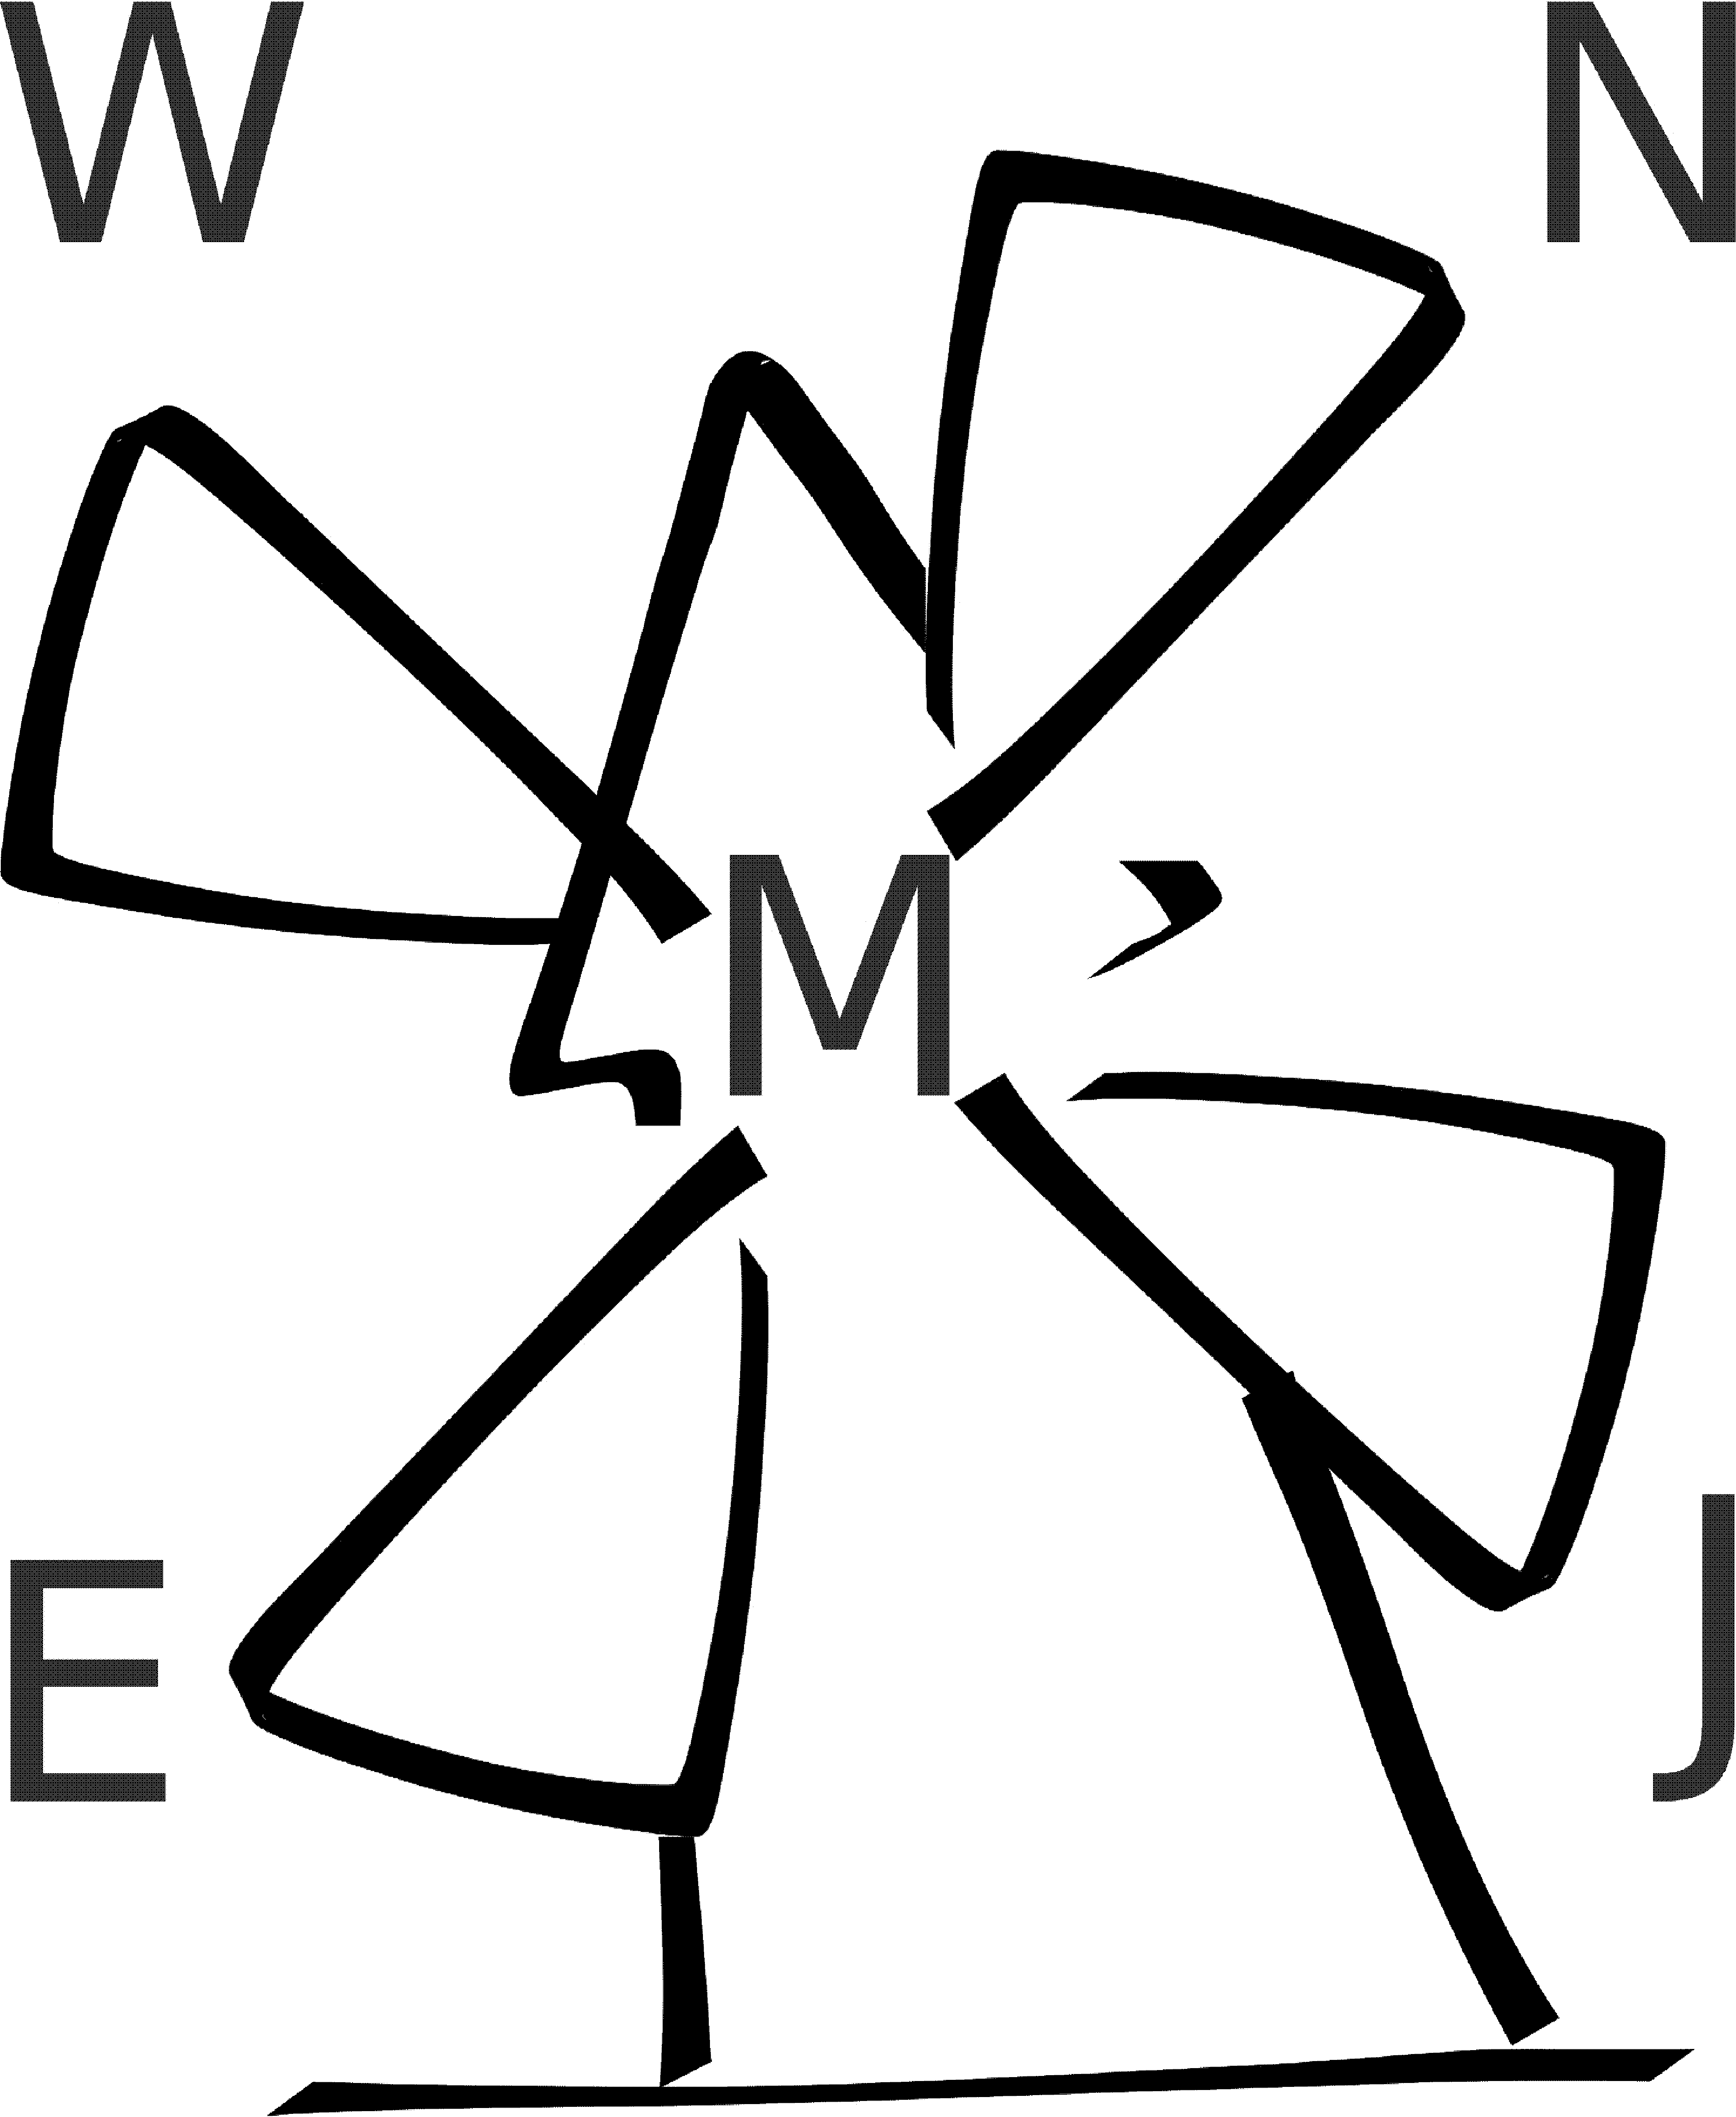
\includegraphics[width=1cm]{ grandMoulinNB }
  }
  \hbox_set_to_wd:Nnn \l_@@_journal_logo_box { 1cm }
  {
    \box_move_down:nn
    {
      \box_ht:N \l_@@_journal_logo_box / 2
      -
      \box_ht:N \l_@@_journal_name_box / 2
    }
    {
      \box_use:N \l_@@_journal_logo_box
    }
  }
  \box_set_ht:Nn \l_@@_journal_logo_box { 0pt }
  \box_set_dp:Nn \l_@@_journal_logo_box { 0pt }
}
%
\newpagestyle{@@_article_title_ps}[]{%
  % \widenhead{\c_zero_dim}{\c_zero_dim}
  \sethead%
  {
    \box_use:N \l_@@_journal_name_box
  }%
  {%
  }%
  {
    \box_use:N \l_@@_journal_logo_box
  }%
  %
  \setfoot%
  {}%
  {\thepage}%
  {}%
}
%    \end{macrocode}
%
% \section{First pages}
%
% At begin of the document, we automatically :
% \begin{itemize}
% \item set the graphic path,
% \item set the page grid if the corresponding option has been passed,
% \item display of the front cover and the inside front cover.
% \end{itemize}
%
%    \begin{macrocode}
\AtBeginDocument{%
  \graphicspath{{\c_@@_issue_images_path_string_tl//}{../\c_@@_issue_images_path_string_tl//}}
  % \glsdisablehyper
}
%    \end{macrocode}
%
% At the begin of document, we automatically switch to
% \begin{itemize}
% \item frontmatter\footnote{Mainly: page numbers in roman.} in the \enquote{issue}
%   version of the class (the first pages are for the table of contents which
%   was decided to be in frontmatter),
% \item mainmatter\footnote{Page numbers in arabic, right page style, right
%   geometry of the page.} in the \enquote{article} version of the class.
% \end{itemize}
%    \begin{macrocode}
\AtBeginDocument{%
%<class-article>    \g_@@_mainmatter_switch_tl
}
%    \end{macrocode}
%
% \section{Options}
%
% In this section, options used by some of the document commands defined by the
% class are treated.
%
%    \begin{macrocode}
%</class|class-article>
%    \end{macrocode}
%
%    \begin{macrocode}
%<*class>
%    \end{macrocode}
%
% \subsection{Journal options}
%
% \begin{macro}{\l_@@_journal_publisher_tl}
% \begin{macro}{\l_@@_journal_address_tl}
% \begin{macro}{\l_@@_journal_phone_tl}
% \begin{macro}{\l_@@_journal_email_tl}
% \begin{macro}{\l_@@_journal_url_tl}
% \begin{macro}{\l_@@_journal_issn_tl}
% \begin{macro}{\l_@@_journal_isbn_tl}
% Some variables which are involved in options are created.
%    \begin{macrocode}
\tl_new:N \l_@@_journal_publisher_tl
\tl_new:N \l_@@_journal_address_tl
\tl_new:N \l_@@_journal_phone_tl
\tl_new:N \l_@@_journal_email_tl
\tl_new:N \l_@@_journal_url_tl
\tl_new:N \l_@@_journal_issn_tl
\tl_new:N \l_@@_journal_isbn_tl
%    \end{macrocode}
% \end{macro}
% \end{macro}
% \end{macro}
% \end{macro}
% \end{macro}
% \end{macro}
% \end{macro}
% \end{macro}
%
% \begin{macro}{publisher}
% \begin{macro}{address}
% \begin{macro}{phone}
% \begin{macro}{email}
% \begin{macro}{url}
% \begin{macro}{issn}
% \begin{macro}{isbn}
% The keys options are created.
%    \begin{macrocode}
\keys_define:nn { nwejm/journalsetup }
{
  publisher .tl_set:N = \l_@@_journal_publisher_tl,
  address .tl_set:N = \l_@@_journal_address_tl,
  phone .tl_set:N = \l_@@_journal_phone_tl,
  email .tl_set:N = \l_@@_journal_email_tl,
  url .tl_set:N = \l_@@_journal_url_tl,
  issn .tl_set:N = \l_@@_journal_issn_tl,
  isbn .tl_set:N = \l_@@_journal_isbn_tl,
%    \end{macrocode}
%
% All these options, when used, must receive a value.
%    \begin{macrocode}
  publisher .value_required:,
  address .value_required:,
  phone .value_required:,
  email .value_required:,
  url .value_required:,
  issn .value_required:,
  isbn .value_required:,
}
%    \end{macrocode}
% \end{macro}
% \end{macro}
% \end{macro}
% \end{macro}
% \end{macro}
% \end{macro}
% \end{macro}
% \end{macro}
%
%    \begin{macrocode}
%</class>
%    \end{macrocode}
%
%    \begin{macrocode}
%<*class|class-article>
%    \end{macrocode}
%
% \subsection{Issues options}
%
% \begin{macro}{\g_@@_issue_number_int}
% \begin{macro}{\g_@@_issue_month_int}
% \begin{macro}{\g_@@_issue_year_int}
% Some variables which are involved in options are created.
%    \begin{macrocode}
\int_new:N \g_@@_issue_number_int
\int_new:N \g_@@_issue_month_int
\int_new:N \g_@@_issue_year_int
\tl_new:N \g_@@_frontcover_image_options_tl
%    \end{macrocode}
% \end{macro}
% \end{macro}
% \end{macro}
%
% \begin{macro}{number}
% \begin{macro}{volume}
% The keys options are created.
%    \begin{macrocode}
\keys_define:nn { nwejm/issuesetup }
{
  number .int_gset:N = \g_@@_issue_number_int,
  volume .int_gset:N = \g_@@_issue_volume_int,
%    \end{macrocode}
%
% All these options, when used, must receive a value.
%    \begin{macrocode}
  volume .value_required:,
%    \end{macrocode}
%
% If "number" option is not used, its initial value is set to $0$.
% number.
%    \begin{macrocode}
  volume .initial:n = 0,
}
%    \end{macrocode}
%
% \end{macro}
% \end{macro}
%
% \subsection{Dates options}
%
% \begin{macro}{received}
% \begin{macro}{accepted}
% \begin{macro}{online}
% Some keys options for article's dates are created:
%    \begin{macrocode}
\keys_define:nn { nwejm/dates }
{
  received   .code:n = {
    \tl_gset:Nn \g_@@_reception_date_tl {#1}
    \bool_gset_true:N \g_@@_date_specified_bool
  },
  accepted   .code:n = {
    \tl_gset:Nn \g_@@_acception_date_tl {#1}
    \bool_gset_true:N \g_@@_date_specified_bool
  },
  online   .code:n = {
    \tl_gset:Nn \g_@@_online_date_tl {#1}
    \bool_gset_true:N \g_@@_date_specified_bool
  },
%    \end{macrocode}
%
% The following options, when used, must receive a value.
%    \begin{macrocode}
  received .value_required:,
  accepted .value_required:,
  online   .value_required:,
}
%    \end{macrocode}
% \end{macro}
% \end{macro}
% \end{macro}
%
% \subsection{Authors options}
%
%    \begin{macrocode}
\quark_new:N \q_@@
\int_new:N \l_author_int
\prop_new:N \g_authors_prop
\prop_new:N \l_affiliations_tagged_prop
\cs_generate_variant:Nn \prop_put_if_new:Nnn { NVn }
\cs_generate_variant:Nn \prop_gput_if_new:Nnn { Nxn }
\cs_generate_variant:Nn \prop_put_if_new:Nnn { NnV }
%    \end{macrocode}
%
% Currently, \Package{expl3} doesn't provide any command that counts the number
% of items of property lists. It should be implemented soonish and, meanwhile,
% Bruno Le Floch provided the following macros (see
% \url{https://github.com/latex3/latex3/issues/293}).
%    \begin{macrocode}
\cs_new:Npn \__@@_prop_count:nn #1#2 { + 1 }
\cs_new:Npn \@@_prop_count:N #1
{ \int_eval:n { 0 \prop_map_function:NN #1 \__@@_prop_count:nn } }
%    \end{macrocode}
%
% \begin{macro}{affiliation}
% \begin{macro}{affiliationtagged}
% The keys options are created.
%    \begin{macrocode}
\NewDocumentCommand \@@_author_affiliation:ww { o u\q_@@ }
{
  \stepcounter{footnote}
  \prop_put_if_new:NVn \l_tmpa_prop {\the\c@footnote} {#2}
  \IfValueT{#1}{%
    \prop_put_if_new:NnV \l_affiliations_tagged_prop {#1} {\the\c@footnote}
  }
}
%
\keys_define:nn { nwejm / authors }
{
  email .tl_gset:N = \g_@@_people_email_tl,
  affiliation .code:n = {%
    \@@_author_affiliation:ww #1 \q_@@
  },
  affiliationtagged .code:n = {%
    \prop_get:NnNTF \l_affiliations_tagged_prop {#1} \l_tmpa_tl
    {%
      \prop_put_if_new:NVn \l_tmpa_prop {\l_tmpa_tl} {}
    }{
      \msg_error:nnn{@@}{Unknown~tag}{#1}
    }
  },
%    \end{macrocode}
%
% All these options, when used, must receive a value.
%    \begin{macrocode}
  affiliation .value_required:,
  affiliationtagged .value_required:,
}
%    \end{macrocode}
% \end{macro}
% \end{macro}
%
% \subsection{New theorem options}
%
%    \begin{macrocode}
\tl_new:N \l_nwejm_newtheorem_style_tl
\keys_define:nn { nwejm / newtheorem }
{
  title .tl_set:N = \l_@@_newtheorem_title_tl,
  title / french .tl_set:N = \l_@@_newtheorem_french_title_tl,
  title / english .tl_set:N = \l_@@_newtheorem_english_title_tl,
  title / german .tl_set:N = \l_@@_newtheorem_german_title_tl,
  title / dutch .tl_set:N = \l_@@_newtheorem_dutch_title_tl,
  title .value_required:,
  title / french .value_required:,
  title / english .value_required:,
  title / german .value_required:,
  title / dutch .value_required:,
  %
  style .choice:,
  style / theorem .code:n = {\tl_set:Nn \l_@@_newtheorem_style_tl {theorem}},
  style / definition .code:n = {\tl_set:Nn \l_@@_newtheorem_style_tl {definition}},
  style / proof .code:n = {\tl_set:Nn \l_@@_newtheorem_style_tl {proof}},
  style / unknown .code:n =
  \msg_error:nnxxx { nwejm } { Unknown~choice }
  { style } % Name of choice key
  { theorem~or~definition~or~proof } % Valid choices
  { \exp_not:n {#1} } % Invalid choice given
}
%    \end{macrocode}
% \end{macro}
% \end{macro}
% \end{macro}
%
% \section{Miscellaneous token lists}
%
% We define some token lists for the long and short forms of the journal.
%    \begin{macrocode}
\tl_new:N \g_@@_nwejm_short_string_tl
\tl_new:N \g_@@_nwejm_string_tl
\tl_gset:Nn \g_@@_nwejm_short_string_tl {
  \cs_if_exist:cTF {texorpdfstring}
  {
    \texorpdfstring{\emph{\c_@@_journal_short_title_string_tl}}{\c_@@_journal_short_title_string_tl}
  }{%
    \emph{\c_@@_journal_short_title_string_tl}
  }%
}
\tl_gset:Nn \g_@@_nwejm_string_tl {
  \cs_if_exist:cTF {texorpdfstring}
  {
    \texorpdfstring{\emph{\c_@@_journal_title_string_tl}}{\c_@@_journal_title_string_tl}
  }{%
    \emph{\c_@@_journal_title_string_tl}
  }%
}
%    \end{macrocode}
%
% We fix some strings for the PDF's metadata .
%    \begin{macrocode}
\tl_new:N \l_@@_pdftitle_string_tl
\tl_new:N \l_@@_pdfauthor_string_tl
\tl_set:Nn \l_@@_pdftile_string_tl {
  \c_@@_journal_title_string_tl\space--\space{}N°\int_use:N\g_@@_issue_number_int
}
\tl_set:Nn \l_@@_pdfauthor_string_tl {
  \g_@@_nwejm_string_tl
}
%    \end{macrocode}
%
%    \begin{macrocode}
\cs_new_protected:Nn \_@@_email:n
  {
    \href{mailto:#1}{\nolinkurl{#1}}%
  }
%    \end{macrocode}
%
% We create a control sequence that populates the bib file.
%    \begin{macrocode}
\tl_new:N \l_@@_crossref_tl
\cs_new_protected:Nn \_@@_populate_bib_file:nn
{
  \int_if_exist:cF {g_@@_#2_int}
  {
    \int_new:c {g_@@_#2_int}
  }
  \int_incr:c {g_@@_#2_int}
  \tl_if_in:nnTF { #2 } { author } {
    \tl_set:Nn \l_@@_crossref_tl {%
      \c_@@_issue_bib_key_tl
      -art-
      \int_use:N \g_@@_articles_int
    }
  } {
    \tl_set:Nn \l_@@_crossref_tl {\c_@@_issue_bib_key_tl}
  }
  \tl_set:Nn \l_@@_people_first_last_name_tl {#1}
  % \tl_show:N \g_@@_article_bib_key_tl
  % \int_show:N \g_@@_articles_int
  \iow_now:Nx \g_@@_bib_out_iow {%
    @article{
      \c_@@_issue_bib_key_tl -#2- \int_use:c {g_@@_#2_int},
      \iow_newline:
      author={\exp_not:V\l_@@_people_first_last_name_tl},
      \iow_newline:
      options={skipbib},
      \iow_newline:
      crossref  = {\l_@@_crossref_tl}
      \iow_newline:
    }
    \iow_newline:
  }%
}
%    \end{macrocode}
%
%    \begin{macrocode}
%</class|class-article>
%    \end{macrocode}
%
%    \begin{macrocode}
%<*class>
%    \end{macrocode}
%
% \section{Functions for specifiying the people involved in the journal}
%
% For this, and thanks to \Pkg{datatool}, we create a database of
% \enquote{people} involved in the journal.
%    \begin{macrocode}
\DTLnewdb{people}
%    \end{macrocode}
%
% Then we create the internal "\_@@_people" function that let us populate the
% "_@@_people" database. Each people will be identified by some identifiers:
% speciality (optional), firstname, lastname, affiliation, email, role.
%    \begin{macrocode}
\cs_new_protected:Nn \_@@_people:nnnnn
{
  \DTLnewrow{people}%
  \DTLnewdbentry{people}{first-last-name}{#1}%
  \DTLnewdbentry{people}{affiliation}{#2}%
  \DTLnewdbentry{people}{country}{#3}%
  \DTLnewdbentry{people}{email}{#4}%
  \DTLnewdbentry{people}{role}{#5}%
  \_@@_populate_bib_file:nn {#1}{#5}
}
%    \end{macrocode}
%
% We create a variant of this control sequence that passes the \emph{values} of
% the variables involved (see
% \url{http://tex.stackexchange.com/a/214284/18401}).
%    \begin{macrocode}
\cs_generate_variant:Nn \_@@_people:nnnnn { nVnVx }
%    \end{macrocode}
%
% \section{Functions for displaying people involved in the journal by role}
%
% We create the function that displays firstname and lastname of people involved
% in the journal by role.
%    \begin{macrocode}
\cs_new_protected:Nn \@@_display_people_by_role:n
{
  \DTLforeach*[\DTLiseq{\l_@@_people_role_tl}{#1}]{people}{%
    \l_@@_firstlastname_tl=first-last-name%
    ,\l_@@_people_affiliation_tl=affiliation%
    ,\l_@@_people_country_tl=country%
    ,\l_@@_people_email_tl=email%
    ,\l_@@_people_role_tl=role%
  }{%
    \tl_if_in:NnTF \l_@@_people_role_tl { editor } {
    \item[
      \_@@_citeauthor_no_firstinits:n {\c_@@_issue_bib_key_tl -#1- \exp_not:V\DTLcurrentindex}%
      ]
      \l_@@_people_affiliation_tl%
        \space%
        (\l_@@_people_country_tl)%
      % ,\space%
      % \_@@_email:n {\l_@@_people_email_tl}
      \DTLiflastrow{%
      }{%
        % \medskip%
      }
    }{
      \tl_if_in:NnTF \l_@@_people_role_tl { author } {
        \footnotesize%
        \noindent%
        \begin{description}[leftmargin=1em,style=nextline]
        \item[%
          \_@@_citeauthor_no_firstinits:n {\c_@@_issue_bib_key_tl -#1- \exp_not:V\DTLcurrentindex}%
          ]
          \tl_if_empty:NF \l_@@_people_affiliation_tl
          {%
            \mbox{}%
            \par%
            \vspace{-2ex}%
            \l_@@_people_affiliation_tl%
          }
          \tl_if_empty:NF \l_@@_people_email_tl
          {%
            \par%
            \_@@_email:n {\l_@@_people_email_tl}
          }
        \end{description}
        \DTLiflastrow{%
        }{
          \DTLpar%
          \medskip%
        }
      }{
        \_@@_citeauthor_no_firstinits:n {\c_@@_issue_bib_key_tl -#1-
          \exp_not:V\DTLcurrentindex}%
        \tl_if_empty:NF \l_@@_people_email_tl
        {
          \space(\_@@_email:n {\l_@@_people_email_tl})
        }
      }
    }
  }
}
%    \end{macrocode}
%
% \section{Displaying the front cover}
%
% We create the variable that displays the front cover.
%    \begin{macrocode}
\tl_new:N \g_@@_display_frontcover_tl%
\tl_gset:Nn \g_@@_display_frontcover_tl {%
  \bool_gset_true:N \g_@@_frontcover_bool
  \pagestyle{@@_frontcover_ps}%
  \exp_after:wN\newgeometry\exp_after:wN{\c_@@_frontcover_geometry_tl}%
  \noindent%
  \bool_if:NTF {\g_@@_cover_bool} {
    \hspace*{-\c_@@_potential_layoutoffset_dim}
  }{
    \hspace*{-2\c_@@_potential_layoutoffset_dim}
  }
  \vfill%
  \noindent%
  \hspace*{10mm}%
  \hspace*{-\c_@@_potential_layoutoffset_dim}
  % \includegraphics[height=22.5mm]{\c_@@_smf_logo_file_string_tl}%
  \vfill%
  \clearpage%
  \bool_gset_false:N \g_@@_frontcover_bool
}
%    \end{macrocode}
%
% \section{Displaying the inside front cover}
%
% We create the variable that displays the inside front cover.
%    \begin{macrocode}
\tl_new:N \g_@@_display_inside_frontcover_tl%
\tl_gset:Nn \g_@@_display_inside_frontcover_tl {%
  \bool_gset_true:N \g_@@_inside_frontcover_bool%
  \pagestyle{@@_inside_frontcover_ps}%
  \exp_after:wN\newgeometry\exp_after:wN{\c_@@_inside_cover_geometry_tl}%
  \footnotesize%
    \begin{multicols*}{2}
      \setlength{\columnsep}{1mm}
      \begin{description}[leftmargin=2em]
      \item[\textsc{\c_@@_editorinchief_string_tl}] \
        \begin{description}[leftmargin=1em]
          \@@_display_people_by_role:n {editorinchief}
        \end{description}
        \bigskip
        \par
      \item[\textsc{\c_@@_associate_editors_string_tl}] \
        \begin{description}[leftmargin=1em]
          \@@_display_people_by_role:n {editor}
        \end{description}
        \bigskip
        \par
      \item[\textsc{\c_@@_field_editor_string_tl}] \
        \begin{description}[leftmargin=1em]
          \@@_display_people_by_role:n {fieldseditor}
        \end{description}
        \bigskip
        \par
      \item[\textsc{\c_@@_managing_editor_string_tl}] \
        \begin{description}[leftmargin=1em]
          \@@_display_people_by_role:n {managingeditor}
        \end{description}
      \end{description}
    \end{multicols*}
  \clearpage%
  \bool_gset_false:N \g_@@_inside_frontcover_bool
  \pagestyle{@@_frontmatter_ps}%
  \exp_after:wN\newgeometry\exp_after:wN{\c_@@_main_geometry_tl}%
}
%    \end{macrocode}
%
% \section{Displaying the inside back cover}
%
% We create the variable that displays the inside back cover.
%    \begin{macrocode}
\tl_new:N \g_@@_display_inside_backcover_tl%
\tl_gset:Nn \g_@@_display_inside_backcover_tl {%
  \bool_gset_true:N \g_@@_inside_backcover_bool%
  \pagestyle{@@_inside_backcover_ps}%
  \exp_after:wN\newgeometry\exp_after:wN{\c_@@_inside_cover_geometry_tl}%
  % \file_if_exist:nT { \c_@@_authors_instructions_file_tl } {%
    \bool_if:NTF {\g_@@_no_inside_backcover_bool} {
      \hbox{}
    }{%
      \small%
        \file_if_exist:nT { \c_@@_authors_instructions_file_tl } {%
          % \begin{multicols}{2}
          %   \setlength{\columnsep}{1mm}
          \file_input:n {\c_@@_authors_instructions_file_tl}
          % \end{multicols}
          % \setlength{\columnseprule}{1pt}
        }
      \begin{description}[leftmargin=1em]
      \item[\c_@@_editorial_secretariat_string_tl{}~:] \ \par%
        % \l_@@_journal_publisher_tl%
        % \par%
        % \space\textendash{}\space%
        \@@_display_people_by_role:n { secretary }\par
        \l_@@_journal_address_tl\par%
        \c_@@_phone_string_tl{}~:~\l_@@_journal_phone_tl{}\par%
        \_@@_email:n {\l_@@_journal_email_tl}
        \newline%
        % \space\textendash{}\space
        \url{\l_@@_journal_url_tl}
      \item[\c_@@_issn_string_tl{}~:] \l_@@_journal_issn_tl
        \tl_if_empty:NF \l_@@_journal_isbn_tl
        {%
        \item[\c_@@_isbn_string_tl{}~:] \l_@@_journal_isbn_tl
        }
        \bool_if:NT {\g_@@_no_inside_backcover_bool} {
        \item[\c_@@_latexclass_string_tl{}~:]
          \@@_display_people_by_role:n { classdesigner }
        \item[\c_@@_printer_string_tl{}~:] \g_@@_printer_text_tl
        }
      \end{description}
      \bool_if:NT {\g_@@_no_inside_backcover_bool} {
        \g_@@_font_designer_text_tl
      }
    }
  % }{%
  %   \hbox{}
  % }
  \bool_gset_false:N \g_@@_inside_backcover_bool
}
%    \end{macrocode}
%
% \section{Displaying the back cover}
%
% We create the variable that displays the back cover.
%    \begin{macrocode}
\tl_new:N \g_@@_display_backcover_tl%
\tl_gset:Nn \g_@@_display_backcover_tl {%
  \bool_gset_true:N \g_@@_backcover_bool
  \pagestyle{@@_backcover_ps}%
  \exp_after:wN\newgeometry\exp_after:wN{\c_@@_backcover_geometry_tl}%
  \file_if_exist:nTF { \c_@@_backcover_page_file_string_tl } {%
    \file_input:n {\c_@@_backcover_page_file_string_tl}
  }{%
    \hbox{}
  }
}
%    \end{macrocode}
%
%    \begin{macrocode}
%</class>
%    \end{macrocode}
%
%    \begin{macrocode}
%<*class|class-article>
%    \end{macrocode}
%
% \section{Displaying the dates}
%
% We create the variable that displays the dates.
%    \begin{macrocode}
\cs_new_protected:Nn \_@@_date:nn
{
  \tl_if_exist:NT {#2}
  {
    \tl_if_empty:NF {#2}
    {
      \tl_if_eq:NNF {\c_@@_date_received_tl} {#1} { \c_@@_dates_separator_tl }
      \tl_mixed_case:n { \exp_args:No \GetTranslation{#1} }
      \c_@@_colon_tl\space
      \DTMdate{#2}%
    }
  }
}
\tl_new:N \g_@@_display_dates_tl%
\tl_gset:Nn \g_@@_display_dates_tl {%
  \footnotesize%
  \_@@_date:nn {\c_@@_date_received_tl}{\g_@@_reception_date_tl}
  \_@@_date:nn {\c_@@_date_accepted_tl}{\g_@@_acception_date_tl}
  \_@@_date:nn {\c_@@_date_online_tl}  {\g_@@_online_date_tl}
  \tl_gclear:N \g_@@_reception_date_tl
  \tl_gclear:N \g_@@_acception_date_tl
  \tl_gclear:N \g_@@_online_date_tl
}
%    \end{macrocode}
%
% \section{Displaying the keywords}
%
% \begin{macro}{\keywords}
% \begin{macro}{\l_@@_keywords_tl}
%   The command for article's keywords is defined: the article's keywords is
%   store in "\l_@@_keywords_tl" for later use.
%    \begin{macrocode}
\seq_new:N \l_@@_keywords_seq
\tl_new:N \l_@@_keywords_tl
\NewDocumentCommand \keywords { m } {
  \seq_clear:N \l_@@_keywords_seq
  \tl_clear:N \l_@@_keywords_tl
  \seq_set_from_clist:Nn \l_tmpa_seq {#1}
  \seq_set_map:NNn \l_@@_keywords_seq \l_tmpa_seq {
    \exp_not:n {
      % \textbf { ##1 } % It is possible to format each of the keywords
      ##1
    }
  }
  \tl_set:Nn \l_@@_keywords_tl { \seq_use:Nn \l_@@_keywords_seq {,~} }
%<class-article>    \hypersetup{pdfkeywords=\l_@@_keywords_tl}
}
%    \end{macrocode}
% \end{macro}
% \end{macro}
%
% \section{Displaying the Mathematical Subject Classification (\textsc{msc})}
%
% \begin{macro}{\msc}
% \begin{macro}{\l_@@_msc_tl}
%   The command for article's \textsc{msc} is defined: the article's \textsc{msc} is
%   store in "\l_@@_msc_tl" for later use.
%    \begin{macrocode}
\seq_new:N \l_@@_msc_seq
\tl_new:N \l_@@_msc_tl
\NewDocumentCommand \msc { m } {
  \seq_clear:N \l_@@_msc_seq
  \tl_clear:N \l_@@_msc_tl
  %
  % does what the name suggests, set a sequence from the clist
  \seq_set_from_clist:Nn \l_tmpa_seq {#1}
  % applies final arg to each element of second seq and stores result in first seq
  \seq_set_map:NNn \l_@@_msc_seq \l_tmpa_seq {
    % \exp_not:n {
      % \textbf { ##1 } % It is possible to format each of the msc
      ##1
    % }
  }
  %
  % \seq_use puts the items from the seq back in the input with ",~" as a separator
  \tl_set:Nn \l_@@_msc_tl {\seq_use:Nn \l_@@_msc_seq {,~}}
%%<class-article>    \hypersetup{pdfmsc=\l_@@_msc_tl}
}
%    \end{macrocode}
% \end{macro}
% \end{macro}
%
% \section{User level commands}
%
% Here, we gather all the user level (public) commands.
%
%    \begin{macrocode}
%</class|class-article>
%    \end{macrocode}
%
%    \begin{macrocode}
%<*class>
%    \end{macrocode}
%
% \subsection{Populating the people involved in the journal}
%
% \begin{macro}{\editorinchief}
% \begin{macro}{\managingeditor}
% \begin{macro}{\fieldseditor}
% \begin{macro}{\editor}
% \begin{macro}{\classdesigner}
% \begin{macro}{\fontdesigner}
% \begin{macro}{\classmaintainer}
% \begin{macro}{\printingservice}
% \begin{macro}{\computerengineer}
% \begin{macro}{\secretary}
%   We define some document-level commands that let the user specify
%   respectively the editor(s) in chief, the fields editor, the managing editor,
%   the editors, the class designer and maintainer(s), etc.
%%   \enquote{R\'{e}dacteur(s) en chef}.
%    \begin{macrocode}
\NewDocumentCommand \editorinchief {mmmm}
{
  \_@@_people:nnnnn {#1}{#2}{#3}{#4}{editorinchief}
}
\NewDocumentCommand \editor {mmmm}
{
  \_@@_people:nnnnn {#1}{#2}{#3}{#4}{editor}
}
\NewDocumentCommand \fieldseditor {mmmm}
{
  \_@@_people:nnnnn {#1}{#2}{#3}{#4}{fieldseditor}
}
\NewDocumentCommand \managingeditor {mmmm}
{
  \_@@_people:nnnnn {#1}{#2}{#3}{#4}{managingeditor}
}
\NewDocumentCommand \classdesigner {mmmm}
{
  \_@@_people:nnnnn {#1}{#2}{#3}{#4}{classdesigner}
}
\NewDocumentCommand \computerengineer {mmmm}
{
  \_@@_people:nnnnn {#1}{#2}{#3}{#4}{computerengineer}
}
\NewDocumentCommand \classmaintainer {mmmm}
{
  \_@@_people:nnnnn {#1}{#2}{#3}{#4}{classmaintainer}
}
\NewDocumentCommand \fontdesigner {mmmm}
{
  \_@@_people:nnnnn {#1}{#2}{#3}{#4}{fontdesigner}
}
\NewDocumentCommand \printingservice {mmmm}
{
  \_@@_people:nnnnn {#1}{#2}{#3}{#4}{printingservice}
}
\NewDocumentCommand \computerassistance {mmmm}
{
  \_@@_people:nnnnn {#1}{#2}{#3}{#4}{computerassistance}
}
\NewDocumentCommand \secretary {mmmm}
{
  \_@@_people:nnnnn {#1}{#2}{#3}{#4}{secretary}
}
%    \end{macrocode}
% \end{macro}
% \end{macro}
% \end{macro}
% \end{macro}
% \end{macro}
% \end{macro}
% \end{macro}
% \end{macro}
% \end{macro}
% \end{macro}
%
% \subsection{Issue setup}
%
% \begin{macro}{\issuesetup}
%   We define the command that lets the user specify the issue setup.
%    \begin{macrocode}
\NewDocumentCommand \issuesetup { m } {
%    \end{macrocode}
%
% Its keys are set (only "number", "month" and "year" are relevant here).
%    \begin{macrocode}
  \keys_set:nn { nwejm/issuesetup } {#1}
%    \end{macrocode}
%
% We fix some of the PDF's metadata .
%    \begin{macrocode}
\hypersetup{pdftitle=\l_@@_pdftitle_string_tl}
\hypersetup{pdfauthor=\l_@@_pdfauthor_string_tl}
%    \end{macrocode}
%
% We use here the fact that, if the "number", "month" or "year" options are not
% used, their corresponding "\g_@@_issue_number_int", "\g_@@_issue_month_int" or
% "\g_@@_issue_year_int" variables are equal to $0$ ($<1$).
%
% First, if "number" is not used, its "\g_@@_issue_number_int" variable is set
% to "\c_@@_first_issue_number_int"\footnote{The number of the first journal's
% issue using the present class.} and a warning is emitted.
%    \begin{macrocode}
  \int_compare:nNnT {\g_@@_issue_number_int}<{1}
  {
    \int_gset:Nn \g_@@_issue_number_int { \c_@@_first_issue_number_int }
    \msg_warning:nnn{nwejm}{Issue~number~needed}{number}
  }
%    \end{macrocode}
%
% If not specified as \refCom{issuesetup}'s key-value options, issue's month and
% year are computed from issue number (which defaults to
% "\c_@@_first_issue_month_int").
%
% \begin{macro}{\c_@@_issue_age_in_months_int}
%   First, if "month" or "year" option is not used (one of the previous
%   variables is $0$ hence their product is $0$ ($<1$)), we compute the issue
%   age in months, useful for both month and year computation.
%    \begin{macrocode}
  \int_compare:nNnT {\g_@@_issue_month_int * \g_@@_issue_year_int}<{1}
  {
    \int_new:N \g_@@_issue_age_in_months_int%
    \int_gset:Nn \g_@@_issue_age_in_months_int
    {
      \c_@@_first_issue_month_int
      + \c_@@_interval_in_months_int
      * ( \int_use:N \g_@@_issue_number_int - \c_@@_first_issue_number_int )
    }
  }
%    \end{macrocode}
% \end{macro}
%
% If the "month" is not used, we replace "\g_@@_issue_month_int" ($=0$) by its
% computed value from the issue number.
%    \begin{macrocode}
  \int_compare:nNnT {\g_@@_issue_month_int}<{1}
  {
    \int_gset:Nn \g_@@_issue_month_int
    {
      \int_mod:nn { \g_@@_issue_age_in_months_int } { 12 }
    }
  }
%    \end{macrocode}
%
% If the "year" is not used, we replace "\g_@@_issue_year_int" ($=0$) by its
% computed value from the issue number.
%    \begin{macrocode}
  \int_compare:nNnT {\g_@@_issue_year_int}<{1}
  {
    \int_new:N \g_@@_issue_age_in_years_int%
    \int_gset:Nn \g_@@_issue_age_in_years_int
    {%
      \int_div_truncate:nn { \g_@@_issue_age_in_months_int } { 12 }
    }%
    \int_gset:Nn \g_@@_issue_year_int
    {
      \g_@@_issue_age_in_years_int + \c_@@_first_issue_year_int
    }
  }%
}
%    \end{macrocode}
% \end{macro}
%
% \subsection{Journal setup}
%
% \begin{macro}{\journalsetup}
%   We define the command that lets the user specify the
%   journal setup. This setup is likely to be rarely changed.
%    \begin{macrocode}
\NewDocumentCommand \journalsetup { m } {
%    \end{macrocode}
%
% Its keys are set (only "publisher", "address", "phone", "email", "url"
% and "issn" are relevant here).
%    \begin{macrocode}
  \keys_set:nn { nwejm/journalsetup } { #1 }
}
%    \end{macrocode}
% \end{macro}
%
% \subsection{\Pkg{Varioref}}
%
% We have to save the extra definitions of the \Pkg{varioref} which currently is
% multilingual aware.
%    \begin{macrocode}
\addto\extrasfrench{%
  \def\reftextfaceafter {page~\reftextvario{ci-contre}{suivante}}%
  \def\reftextfacebefore{page~\reftextvario{ci-contre}%
    {pr\’ec\’edente}}%
  \def\reftextafter
  {page~suivante}%
  \def\reftextbefore
  {page~pr\’ec\’edente}%
  \def\reftextcurrent
  {de~la~pr\’esente~page}%
  \def\reftextfaraway#1{page~\pageref{#1}}%
  \def\reftextpagerange#1#2{pages~\pageref{#1}--\pageref{#2}}%
  \def\reftextlabelrange#1#2{\ref{#1}~\‘a~\ref{#2}}%
}
\addto\extrasngerman{%
  \def\reftextfaceafter {auf~der~n\"achsten~Seite}%
  \def\reftextfacebefore{auf~der~vorherigen~Seite}%
  \let\reftextafter     \reftextfaceafter
  \let\reftextbefore    \reftextfacebefore
  \def\reftextcurrent   {auf~dieser~Seite}%
  \def\reftextfaraway#1{auf~Seite~\pageref{#1}}%
  \def\reftextpagerange#1#2{auf~den~Seiten~\pageref{#1}--\pageref{#2}}%
  \def\reftextlabelrange#1#2{\ref{#1}~bis~\ref{#2}}%
}
\addto\extrasdutch{%
  \def\refpagename{pagina}%
  \def\reftextfaceafter {op~de~\reftextvario{rechter~\refpagename}%
    {\refpagename\ hiernaast}}%
  \def\reftextfacebefore{op~de~\reftextvario{linker~\refpagename}%
    {\refpagename\ hiernaast}}%
  \def\reftextafter     {op~de~\reftextvario{volgende~\refpagename}%
    {\refpagename\ hierna}}%
  \def\reftextbefore    {op~de~\reftextvario{vorige~\refpagename}%
    {\refpagename\ hiervoor}}%
  \def\reftextcurrent   {op~deze~\refpagename}%
  \def\reftextfaraway#1{op~\refpagename\space\pageref{#1}}
}
\addto\extrasenglish{%
  \def\reftextfaceafter {on~the~\reftextvario{facing}{next}~page}%
  \def\reftextfacebefore{on~the~\reftextvario{facing}{preceding}~page}%
  \def\reftextafter     {on~the~\reftextvario{following}{next}~page}%
  \def\reftextbefore    {on~the~\reftextvario{preceding}{previous}~page}%
  \def\reftextcurrent   {on~\reftextvario{this}{the~current}~page}%
  \def\reftextfaraway#1{on~page~\pageref{#1}}%
  \def\reftextpagerange#1#2{on~pages~\pageref{#1}--\pageref{#2}}%
  \def\reftextlabelrange#1#2{\ref{#1}~to~\ref{#2}}%
}
%    \end{macrocode}
% \end{macro}
%
%    \begin{macrocode}
%</class>
%    \end{macrocode}
%
%    \begin{macrocode}
%<*class|class-article>
%    \end{macrocode}
%
% \subsection{Dates setup}
%
% \begin{macro}{\dates}
%   We define the command that lets the user specify the issue setup.
%    \begin{macrocode}
\NewDocumentCommand \dates { m } {
  \keys_set:nn { nwejm/dates } { #1 }
}
%    \end{macrocode}
% \end{macro}
%
% \subsection{Input variant}
%
% We create a variant of the "\input" macro to be use for the input of each
% article: it starts a new \package{biblatex}'s "refsection" and reset to zero
% some counters.
%    \begin{macrocode}
\NewDocumentCommand \inputarticle { O{english} m } {%
  \newrefsection
  \tl_if_eq:nnTF { #1 } { german } {%
    \selectlanguage{ngerman}
  }{
    \selectlanguage{#1}
  }%
  \inputfrom{./}{#2}
  \setcounter{footnote}{0}
  \setcounter{section}{0}
  \setcounter{figure}{0}
  \setcounter{table}{0}
  \setcounter{equation}{0}
  \setcounter{theorem}{0}
  \setcounter{corollary}{0}
  \setcounter{conjecture}{0}
  \setcounter{proposition}{0}
  \setcounter{lemma}{0}
  \setcounter{axiom}{0}
  \setcounter{definition}{0}
  \setcounter{remark}{0}
  \setcounter{example}{0}
  \setcounter{notation}{0}
%    \end{macrocode}
% We reset all acronyms entries.
%    \begin{macrocode}
  \glsresetall
  \selectlanguage{english}
}
%    \end{macrocode}
%
% \section{(Re)Definition of document commands that identify the article}
%
% The names of the authors of the different articles will appear at several
% places, and notably in the table of contents where first and middle names have to
% be rendered as initials. Because automatically rendering initials is a complex task
% already provided by \Pkg{biblatex}, we will create a \file{.bib} file
% containing "article" entries for each article of the \nwejm{} journal.
%
% This can be done only at the beginning of the document, in order to know the
% characteristics of the current issue.
%    \begin{macrocode}
\AtBeginDocument{%
%    \end{macrocode}
%
% We first create a token list containing the date of the current issue formated
% as required by \pkg{biblatex} (the month issue needs a leading zero if it is
% $<10$).
%    \begin{macrocode}
\tl_new:N \g_@@_bib_issue_date_tl
\tl_gset:Nn
\g_@@_bib_issue_date_tl {
  \int_use:N \g_@@_issue_year_int -
  \int_compare:nNnT {\g_@@_issue_month_int}<{10}
  {
    0
  }
  \int_use:N \g_@@_issue_month_int
}
%    \end{macrocode}
%
% We will populate the bibiliographic file of the current issue with the current
% issue (as "@periodical" entry type).
%    \begin{macrocode}
  \iow_now:Nx \g_@@_bib_out_iow {%
    @periodical{\c_@@_issue_bib_key_tl,\iow_newline:
      issuetitle   = {\exp_not:f\c_@@_journal_title_string_tl},\iow_newline:
      date         = {\g_@@_bib_issue_date_tl},\iow_newline:
      number       = \int_use:N \g_@@_issue_number_int,\iow_newline:
      % issn         = {\l_@@_journal_issn_tl},\iow_newline:
      options      = {skipbib}\iow_newline:
    }
    \iow_newline:
  }%
}
%    \end{macrocode}
%
% \begin{macro}{\title}
% \begin{macro}{\g_@@_title_tl}
%   The command for article's title is redefined: the full \enquote{article's
%   title} is store in "\g_@@_title_tl" for later use.
%    \begin{macrocode}
\tl_new:N \g_@@_title_tl
\RenewDocumentCommand \title { o m } {
%    \end{macrocode}
%
% We don't want the (next) title to appear in the headers of the preceding
% article.
%    \begin{macrocode}
  \cleardoublepage
%    \end{macrocode}
%
% We increment the "\g_@@_articles_int" integer that counts the number of
% articles in order to provide for each of them a unique bibliographic key.
%    \begin{macrocode}
  \int_gincr:N \g_@@_articles_int
  \tl_gclear:N \g_@@_short_title_tl
  \tl_gclear:N \g_@@_short_subtitle_tl
  %
  \IfNoValueF {#1}
  {
    \tl_gset:Nn \g_@@_short_title_tl {#1}
  }
  \tl_gset:Nn \g_@@_title_tl {#2}
  \tl_if_empty:NT \g_@@_short_title_tl {%
    \tl_gset_eq:NN \g_@@_short_title_tl \g_@@_title_tl
  }
}
%    \end{macrocode}
% \end{macro}
% \end{macro}
%
% \begin{macro}{\subtitle}
% \begin{macro}{\g_@@_subtitle_tl}
%   The command for article's subtitle is redefined: the full and short
%   \enquote{article's subtitles} are store in "\g_@@_subtitle_tl" and
%   "\g_@@_short_subtitle_tl" for later use.
%    \begin{macrocode}
\tl_new:N \g_@@_subtitle_tl
\NewDocumentCommand \subtitle { o m } {
  \IfNoValueF {#1}
  {
    \tl_gset:Nn \g_@@_short_subtitle_tl {#1}
  }
  \tl_gset:Nn \g_@@_subtitle_tl {#2}
  \tl_if_empty:NT \g_@@_short_subtitle_tl {%
    \tl_gset_eq:NN \g_@@_short_subtitle_tl \g_@@_subtitle_tl
  }
}
%    \end{macrocode}
% \end{macro}
% \end{macro}
%
% \begin{macro}{\author}
% The command for article's author (including its affiliation) is redefined.
%    \begin{macrocode}
\RenewDocumentCommand \author { O{} m } {
%    \end{macrocode}
%
% We don't want the (next) authors to appear in the headers of the preceding
% article.
%    \begin{macrocode}
  \cleardoublepage
%    \end{macrocode}
%
  \int_incr:N \l_author_int
  \prop_gput_if_new:Nxn \g_authors_prop {author_\int_use:c {l_author_int}} {#2}
  \IfNoValueF {#1}
  {
    \keys_set:nn { nwejm/authors } { #1 }
  }
  \prop_set_eq:cN {l_author_ \int_use:c {l_author_int} _affiliations_prop} \l_tmpa_prop
  \prop_clear:N \l_tmpa_prop
  \_@@_populate_bib_file:nn {#2}{author-art-\int_use:N \g_@@_articles_int}
  \tl_if_empty:NTF \l_@@_people_first_last_names_tl {%
    \tl_put_right:Nn
    \l_@@_people_first_last_names_tl
    {#2}
  }{
    \tl_put_right:Nn
    \l_@@_people_first_last_names_tl
    {~and~#2}
  }
}
%    \end{macrocode}
% \end{macro}
%
% We create a stream in order to write a bibliographic file
%    \begin{macrocode}
\iow_new:N \g_@@_bib_out_iow
\ior_new:N \g_@@_bib_out_ior
\tl_new:N \g_@@_bib_out_tl
\file_if_exist:nTF { \c_@@_issue_bib_path_string_tl }
{
  \ior_open:Nn \g_@@_bib_out_ior { \c_@@_issue_bib_path_string_tl }
  \ior_str_map_inline:Nn \g_@@_bib_out_ior
  { \tl_gput_right:Nn \g_@@_bib_out_tl {#1 \par } }
  \ior_close:N \g_@@_bib_out_ior
}{
  \typeout{no file! rerun}
}
\iow_open:Nn \g_@@_bib_out_iow { \c_@@_issue_bib_path_string_tl }
%    \end{macrocode}
%
% \begin{environment}{abstract}
%   The environment for article's abstract.
%    \begin{macrocode}
\tl_new:N \g_@@_abstract_body_tl
\NewDocumentEnvironment{abstract}{}
  {\CollectAbstract}
  {\endCollectAbstract}
\NewEnviron{CollectAbstract}
  {
    \tl_gset_eq:NN \g_@@_abstract_body_tl \BODY
  }
%    \end{macrocode}
% \end{environment}
%
% \section{Definition of a private front and main matter switches}
%
% A private "\_@@_frontmatter_switch_tl" switch is defined in order to
% automatically insert some settings.
%    \begin{macrocode}
\tl_new:N \g_@@_frontmatter_switch_tl%
\tl_gset:Nn \g_@@_frontmatter_switch_tl {
  \bool_gset_true:N  \g_@@_frontmatter_bool
  \frontmatter
  \pagestyle{@@_frontmatter_ps}%
  \exp_after:wN\newgeometry\exp_after:wN{\c_@@_main_geometry_tl}%
}
%    \end{macrocode}
%
% A private "\_@@_mainmatter_switch_tl" switch is defined in order to
% automatically insert some settings.
%    \begin{macrocode}
\tl_new:N \g_@@_mainmatter_switch_tl%
\tl_gset:Nn \g_@@_mainmatter_switch_tl {
  \bool_gset_false:N \g_@@_frontmatter_bool
  \bool_gset_true:N \g_@@_mainmatter_bool
  \mainmatter
  % \SetParskip{\c_@@_mainmatter_parskip_skip}
  \pagestyle{@@_mainmatter_ps}%
  \exp_after:wN\newgeometry\exp_after:wN{\c_@@_main_geometry_tl}%
}
%    \end{macrocode}
%
% \section{Definition of the acknowledgments}
%
%    \begin{macrocode}
\tl_new:N \g_@@_article_acknowledgments_tl%
\cs_new_protected:Nn \@@_article_acknowledgments:n
{
  \tl_gset:Nn \g_@@_article_acknowledgments_tl { #1 }
}
\NewDocumentCommand \acknowledgments { m } {
  \@@_article_acknowledgments:n {#1}
}
%    \end{macrocode}
%
% \section{Definition of the title command}
%
% We create two token lists that will contain:
% \begin{enumerate}
% \item the unique bibliographic key,
% \item the "author" value of the bibliographic entry,
% \end{enumerate}
%  of the current article.
%    \begin{macrocode}
\tl_new:N \g_@@_article_bib_key_tl%
\tl_new:N \l_@@_people_first_last_names_tl
\tl_new:N \g_@@_authors_first_last_names_tl%
\tl_new:N \g__@@_citeauthor_no_firstinits%
\tl_new:N \g_@@_citeauthor_tl%
\int_new:N \g_@@_author_s_number_current_article_int%
%
\cs_new_protected:Nn \_@@_citeauthor_no_firstinits:n {%
  \tl_gset:Nn \g_@@_citeauthor_tl {%
    \DeclareNameAlias{labelname}{default}%
    \group_begin:
    \togglefalse{blx@firstinits}%
    \citeauthor{#1}
    \group_end:
  }%
  \cs_if_exist:cTF {texorpdfstring}
  {
    \texorpdfstring{\g_@@_citeauthor_tl}{}
  }{%
    \g_@@_citeauthor_tl
  }%
}
%    \end{macrocode}
%
% In the following "\maketitle" document level macro, we will need to display
% the list the authors of the current article, not as a comma separated list
% (default "\citeauthor" \pkg{biblatex}'s macro behavior), but as an itemized
% list. For this, we create the "\_@@_itemized_citeauthor" internal function
% that will make use of "\citeauthor" where "\multinamedelim" and
% "\finalnamedelim" will be patched into "\item". As we don't want to globally
% alter the behavior of these macros, we first store their original meanings in
% some private control sequence:
%    \begin{macrocode}
\cs_set_eq:NN \_@@_orig_multinamedelim \multinamedelim
\cs_set_eq:NN \_@@_orig_finalnamedelim \finalnamedelim
\cs_new_protected:Nn \_@@_maketitle_citeauthor:n
{
  \restorecommand\mkbibnamelast
  \def\multinamedelim  {\hskip 1em \@plus.17fil}%
  \cs_set_eq:NN \finalnamedelim \multinamedelim
  \AtNextCitekey{\defcounter{maxnames}{100}}
  \group_begin:
  \DeclareNameAlias{labelname}{default}%
  \togglefalse{blx@firstinits}%
  \citeauthor{#1}
  \group_end:
  \cs_set_eq:NN \multinamedelim \_@@_orig_multinamedelim
  \cs_set_eq:NN \finalnamedelim \_@@_orig_finalnamedelim
  \protected\def\mkbibnamelast#1{%
    \textsc{\textnohyphenation{#1}}}%
}
\cs_new_protected:Nn \@@_display_author:n
{
  \seq_clear:N \l_tmpa_seq
  \prop_get:NnN \g_authors_prop {author_#1} \l_tmpa_tl
  \prop_map_inline:cn {l_author_ #1 _affiliations_prop} {
    \seq_put_right:Nx \l_tmpa_seq { ##1 }
  }
  \seq_sort:Nn \l_tmpa_seq
  {
    \int_compare:nNnTF { ##1 } > { ##2 }
    { \sort_reversed: }
    { \sort_ordered: }
  }
  \mbox{%
    \_@@_citeauthor_no_firstinits:n {\c_@@_issue_bib_key_tl -author-art- \int_use:N \g_@@_articles_int-#1}
  }
  \seq_map_inline:Nn \l_tmpa_seq {
    \prop_get:cnN {l_author_ #1 _affiliations_prop} {##1} \l_tmpb_tl
    \footnotemark[##1]
    \tl_if_empty:NF \l_tmpb_tl
    {
      \footnotetext[##1]{\l_tmpb_tl}
    }
  }
  \hskip 1em plus .17fil
}
%    \end{macrocode}
%
% We declare two token list which will used in the next (re)definition.
%    \begin{macrocode}
\tl_new:N \l_@@_bullet_and_rule_tl
\tl_new:N \l_@@_authors_box_tl
\tl_new:N \l_@@_abstract_box_tl
\tl_new:N \l_@@_bullet_and_rule_odd_tl
\tl_new:N \l_@@_bullet_and_rule_even_tl
\tl_new:N \l_@@_title_box_tl
\tl_new:N \g_@@_title_for_toc_tl
%    \end{macrocode}
%
% \begin{macro}{\_@@_maketitle}
%   The command that \emph{makes} the title is redefined.
%    \begin{macrocode}
\RenewDocumentCommand \maketitle { } {
%    \end{macrocode}
%
% We enforce all the previous floats to be processed before a new article starts
% (this is already done in "acknowledgments"environment but is repeated here if
% what is before provides floats but  not acknowledgments).
%    \begin{macrocode}
%<class>      \FloatBarrier%
%    \end{macrocode}
%
% We store the unique bibliographic key of the current article in the
% "\g_@@_article_bib_key_tl" token list.
%    \begin{macrocode}
\tl_gset:Nn \g_@@_article_bib_key_tl {%
  \c_@@_issue_bib_key_tl
  -art-
  \int_use:N \g_@@_articles_int
}
%    \end{macrocode}
%
% We will populate the bibiliographic file of the current issue with the current
% article (title, author(s) and a fixed part giving by the issue number, journal
% title and date).
%
% We now populate the bibiliographic file.
%    \begin{macrocode}
\tl_if_empty:NF \g_@@_title_tl {%
  \iow_now:Nx \g_@@_bib_out_iow {%
    @article{
      \g_@@_article_bib_key_tl,
      \iow_newline:
      title={\exp_not:V\g_@@_title_tl},
      \iow_newline:
      \tl_if_empty:NF \g_@@_subtitle_tl {%
        subtitle={\exp_not:V\g_@@_subtitle_tl},
        \iow_newline:
      }
      \tl_if_eq:NNF { \g_@@_short_title_tl } { \g_@@_title_tl } {%
        shorttitle={\exp_not:V\g_@@_short_title_tl},
        \iow_newline:
      }%
      \tl_if_empty:NF \l_@@_people_first_last_names_tl
      {
        author={\exp_not:V\l_@@_people_first_last_names_tl},
        \iow_newline:
      }
      options={skipbib},
      \iow_newline:
      crossref  = {\c_@@_issue_bib_key_tl}
    }
    \iow_newline:
  }%
  % \tl_clear:N \l_@@_people_first_last_names_tl
}%
%
\tl_set:Nn \l_@@_authors_box_tl
{%
  \bool_if:nTF { \tl_if_empty_p:N \l_@@_people_first_last_names_tl }
  {
    \mbox{}
  }
  {
    \int_set:Nn \l_tmpa_int { \@@_prop_count:N \g_authors_prop}
    \normalsize%
    \int_step_inline:nnnn {1}{1}{\l_tmpa_int} {
      \@@_display_author:n {##1}
    }
    \prop_gclear:N \g_authors_prop
  }
}
%    \end{macrocode}
%
% We clear the tagged affiliations (henece their scope is the current article).
%    \begin{macrocode}
\int_zero:N \l_author_int
\prop_clear:N \l_affiliations_tagged_prop
%    \end{macrocode}
%
%    \begin{macrocode}
\tl_set:Nn \l_@@_dates_box_tl
{%
  \g_@@_display_dates_tl
}
%
\tl_set:Nn \l_@@_keywords_box_tl
{%
  \noindent
  {
    \bfseries
    \tl_mixed_case:n{
      \GetTranslation{plural-keyword}
      \c_@@_colon_tl
    }
  }
  \space\l_@@_keywords_tl.
}
\tl_set:Nn \l_@@_msc_box_tl
{%
  \noindent\textbf{\c_@@_msc_string_tl}\c_@@_colon_tl\space\l_@@_msc_tl.
}
\tl_set:Nn \l_@@_abstract_box_tl
{%
  \mbox{}
  \par%
  \vskip .5em%
  \tl_if_empty:NTF \g_@@_abstract_body_tl
  {%
    \msg_warning:nn{nwejmart}{No~abstract}
  }%
  {%
    \small
    \begin{center}%
      {\bfseries \abstractname\vspace{-.5em}\vspace{\z@}}%
    \end{center}%
    \begin{quotation}
      \g_@@_abstract_body_tl
    \end{quotation}
  }
}%
%    \end{macrocode}
%
%    \begin{macrocode}
\tl_set:Nn \g_@@_partial_title_for_toc_tl
{
  \tl_if_empty:NTF \g_@@_short_title_tl {%
    \g_@@_title_tl%
  }{
    \g_@@_short_title_tl%
  }
  \bool_if:nF { \tl_if_empty_p:N \g_@@_short_subtitle_tl }
  {
    \space\textendash{}\space\g_@@_short_subtitle_tl
  }
}
%    \end{macrocode}
%
% For the article's class, the article's title and (if any) subtitle are added
% to the ×pdftitle× PDF's metadata.
%    \begin{macrocode}
%<class-article>    \hypersetup{pdftitle=\g_@@_partial_title_for_toc_tl}
%    \end{macrocode}
%
%    \begin{macrocode}
\tl_set:Nn \g_@@_title_for_toc_tl
{
  \g_@@_partial_title_for_toc_tl
  \bool_if:nF { \tl_if_empty_p:N \l_@@_people_first_last_names_tl }
  {
    \textsl{
      \cs_if_exist:cTF {texorpdfstring}
      {
        \texorpdfstring{%
          \space\textendash{}\space\citeauthor{\g_@@_article_bib_key_tl}
        }{}
      }{%
        \space\textendash{}\space\citeauthor{\g_@@_article_bib_key_tl}
      }%
    }
  }
}
%    \end{macrocode}
%
% The article's titles are produced thanks to the ×\chapter× which is
% unnumbered (otherwise the corresponding bookmark is numbered), but not through
% the starred version of ×\chapter× (because we need its -- alternative title in
% the TOC).
%    \begin{macrocode}
  \setsecnumdepth{none}
%<class-article> \bookmarksetup{depth=-2}

  \chapter[\g_@@_title_for_toc_tl]{%
    \LARGE%
    \g_@@_title_tl
    \tl_if_empty:NF \g_@@_subtitle_tl {%
      \\[1ex]%
      \Large%
      \g_@@_subtitle_tl
    }\\[2ex]%
    \l_@@_authors_box_tl%
    \bool_if:NT {\g_@@_date_specified_bool}
    {
      \\[2ex]
      \l_@@_dates_box_tl
    }
    \\[-4ex]
  }
  \bool_gset_false:N \g_@@_date_specified_bool
  \bookmarksetup{depth=subsection}
  \setsecnumdepth{subsection}
%    \end{macrocode}
%
% We want header of the article's titles pages.
%    \begin{macrocode}
  \thispagestyle{@@_article_title_ps}%
%
\l_@@_abstract_box_tl%
\normalsize
\tl_if_empty:NTF \l_@@_keywords_tl {
  \msg_warning:nn{nwejmart}{No~keyword}
}{
  \l_@@_keywords_box_tl
  \par%
  \vskip .5em%
}
\tl_if_empty:NTF \l_@@_msc_tl {
  \msg_warning:nn{nwejmart}{No~MSC}
}{
  \l_@@_msc_box_tl
  \par%
  \vskip .5em%
}
%<class-article> \hypersetup{pdfauthor=\l_@@_people_first_last_names_tl}
%
\tl_gclear:N \g_@@_title_tl
\tl_gclear:N \g_@@_subtitle_tl
\tl_gclear:N \g_@@_title_for_toc_tl
\tl_gclear:N \g_@@_abstract_body_tl
%    \end{macrocode}
%
% We clear the authors database from the possible previous article.
%    \begin{macrocode}
  \tl_gclear:N \g_@@_people_affiliation_tl
  \tl_gclear:N \g_@@_people_email_tl
  \tl_clear:N \l_@@_people_first_last_names_tl%
}
%    \end{macrocode}
% \end{macro}
%
% We load the configuration file, which has to be located in the \TeX{} search
% path: at least one such a file is provided by the class and located in the
% same directory as the class file. This file is loaded at the end of preamble
% instead of begin of the document in order some settings needed in preamble are
% taken in account.
%    \begin{macrocode}
%<class>\AtEndPreamble{\file_input:n {\c_@@_configuration_file_string_tl}}
%    \end{macrocode}
%
% \subsection{Miscellaneous}
%
% We fix the \pkg{csquotes}' quotes for PDF strings.
%    \begin{macrocode}
\DeclarePlainStyle{«~}{~»}{`}{'}
%    \end{macrocode}
%
% We change the default settings of the floats placement.
%    \begin{macrocode}
\setcounter{topnumber}{3}
\renewcommand{\topfraction}{0.8}
%    \end{macrocode}
%
% We change the default vertical space between text and footnotes.
%    \begin{macrocode}
\addtolength{\skip\footins}{.25\baselineskip}
%    \end{macrocode}
%
% We change the default horizontal space between columns in multicolumn mode.
%    \begin{macrocode}
\setlength{\columnsep}{7mm}%
%    \end{macrocode}
%
% We change the way the section counter is displayed (the chapter should not appear).
%    \begin{macrocode}
\renewcommand{\thesection}{\arabic{section}}%
%    \end{macrocode}
%
% In case \Pkg{siunitx} is loaded, we make it follow the French rules.
%    \begin{macrocode}
\@ifpackageloaded{siunitx}{%
  \addto\extrasenglish{\sisetup{locale = UK}}
  \addto\extrasfrench{\sisetup{locale = FR}}
  \addto\extrasngerman{\sisetup{locale = DE}}
  \addto\extrasgerman{\sisetup{locale = DE}}
  \addto\extrasdutch{%
    \sisetup{%
      exponent-product      = \ensuremath { \times } ,
      inter-unit-product    = \,                     ,
      output-decimal-marker = { , }
    }%
  }
  \sisetup{detect-all}
}
%    \end{macrocode}
%
% \subsection{Redefinition of heading commands}
%
% We redefine the heading commands (×\section× and ×\subsection×, not below as
% the corresponding headings are not numbered) in order the starred versions
% make use of ×\setsecnumdepth{none}× from \Pkg{tocvsec2} and hence save the
% user from having to add the ugly ×\addcontentsline× trick. Here,
% ×\AfterPreamble× is necessary to delay the redefinition when \Pkg{titlesec}
% has done its own.
%
%    \begin{macrocode}
\cs_set_eq:NN \_@@_section \section
\cs_set_eq:NN \_@@_subsection \subsection
\cs_set_eq:NN \_@@_subsubsection \subsubsection
\AfterPreamble{%
  \RenewDocumentCommand \section { s o m } {%
    \IfBooleanTF {#1}
    {
      \setsecnumdepth{none}%
    }
    {
      \resetsecnumdepth*%
    }
    \IfNoValueTF{#2}{\_@@_section{#3}}{\_@@_section[#2]{#3}}
  }
  \RenewDocumentCommand \subsection { s o m } {%
    \IfBooleanT {#1}
    {
      \setsecnumdepth{none}%
    }
    \IfNoValueTF{#2}{\_@@_subsection{#3}}{\_@@_subsection[#2]{#3}}
  }
  \RenewDocumentCommand \subsubsection { s o m } {%
    \IfBooleanT {#1}
    {
      \setsecnumdepth{none}%
    }
    \IfNoValueTF{#2}{\_@@_subsubsection{#3}}{\_@@_subsubsection[#2]{#3}}
  }
}
%    \end{macrocode}
%
% \section{Miscellaneous private commands specific to the journal}
%
% We create miscellaneous private commands specific to the journal.
%
% Command for centuries.
%    \begin{macrocode}
\int_new:N \l_@@_abs_int
%
\cs_new_protected:Nn \_@@_ordinalnum_suffix:n
{
  \int_set:Nn \l_@@_abs_int {\int_abs:n {#1}}
  \ifcurrentbaselanguage{english}{
    \int_use:N \l_@@_abs_int
    \int_set:Nn \l_tmpa_int {\int_mod:nn {\l_@@_abs_int} {\c_one_hundred}}
    \int_case:nnF
    { \l_tmpa_int }
    {
      { \c_eleven }   { \fmtord{th} }
      { \c_twelve }   { \fmtord{th} }
      { \c_thirteen } { \fmtord{th} }
    }{
      \int_set:Nn \l_tmpb_int {\int_mod:nn {\l_@@_abs_int} {\c_ten}}
      \int_case:nnF
      { \l_tmpb_int }
      {
        { \c_zero }   { \fmtord{th} }
        { \c_one }   { \fmtord{st} }
        { \c_two }   { \fmtord{nd} }
        { \c_three } { \fmtord{rd} }
      }{
        \fmtord{th}
      }
    }
  }{
    \ifcurrentbaselanguage{dutch}{
      \int_use:N \l_@@_abs_int
      e
    }{
      \textsc{\int_to_roman:n {\int_abs:n {#1}}}
      \ifcurrentbaselanguage{french}{
        \int_compare:nNnTF { \l_@@_abs_int } = { 1 }{\fmtord{er}}{\fmtord{e}}
      }{
        \ifcurrentbaselanguage{german}{
          .
        }{
          \ifcurrentbaselanguage{ngerman}{
            .
          }{
          }
        }
      }
    }
  }
}
%
\cs_new_protected:Nn \_@@_century_suffix:n
{
  \space{}
  \GetTranslation{century}%
  \int_compare:nNnT { #1 } < { 0 }{
    \space
    \GetTranslation{before-christ}
  }{
  }
}
%    \end{macrocode}
%
% \section{Miscellaneous (re)definitions}
%
% We gather here miscellaneous redefinitions.
%
% \begin{macro}{\century}
%   In case of \enquote{before-christ} translation usually ending with a period
%   (in case of abbreviation), we add a period just after it, but only if the
%   character following the "\century" macro is not a period itself.
%    \begin{macrocode}
\NewDocumentCommand \century { s m } {%
  \_@@_ordinalnum_suffix:n {#2}%
  \IfBooleanTF {#1}
  {
    \int_compare:nNnT { #2 } < { 0 }{
      \_@@_century_suffix:n {#2}%
    }
  }{
    \_@@_century_suffix:n {#2}%
  }
  \int_compare:nNnT { #2 } < { 0 }{
    \ifcurrentbaselanguage{english}{%
    }{
      \@ifnextchar.%
      {
      }{
        .\xspace
      }%
    }
  }
}
%    \end{macrocode}
% \end{macro}
%
% \begin{macro}{\aside}
%    \begin{macrocode}
\NewDocumentCommand \aside { s m } {%
  \IfBooleanTF {#1}
  {
    \c_@@_aside_string_tl{}~#2
  }
  {
    \c_@@_aside_string_tl{}~#2~\c_@@_aside_string_tl
  }
}
%    \end{macrocode}
% \end{macro}
%
% \begin{macro}{\ie}
% \begin{macro}{\Ie}
%    \begin{macrocode}
\NewDocumentCommand \ie { s } {%
  \IfBooleanTF {#1}
  {
    \GetTranslation{idest}
  }
  {
    \GetTranslation{ie}
    \@ifnextchar.%
    {
    }{
      .\xspace
    }%
  }
}
\NewDocumentCommand \Ie { s } {%
  \IfBooleanTF {#1}
  {
    \GetTranslation{Idest}
  }
  {
    \GetTranslation{Ie}
    \@ifnextchar.%
    {
    }{
      .\xspace
    }%
  }
}
%    \end{macrocode}
% \end{macro}
% \end{macro}
%
% \subsection{Vectors}
%
% Vectors, even written with "\vec", are typeset with \pkg{esvect}'s "\vv":
%    \begin{macrocode}
\RenewDocumentCommand \vec { m } {
  \vv{#1}
}
%    \end{macrocode}
%
% \subsection{Usual theorems and the like}
%
% Some usual theorems and the like are defined, thanks to \Pkg{thmtools}. First,
% we define a private function "\_@@_new_theorem" that defines:
% \begin{enumerate}
% \item a new (private, \pkg{thmtools}) theorem with 4 arguments:
%   \begin{enumerate}
%   \item name of the (private) \pkg{thmtools} theorem,
%   \item French title for this theorem,
%   \item English title for this theorem.
%   \end{enumerate}
% \item a public environment based on this private theorem with a the usual
%   syntax of \pkg{amsthm} theorems, except it has an optional argument for
%   possible additional options to the default styles ("theorem" or
%   "definition").
% \end{enumerate}
%
% Then, we define a public command, similar to "\newtheorem", based on
% "\_@@_new_theorem", that lets the user define his own theorems:
%    \begin{macrocode}
\cs_new_protected:Nn \_@@_new_theorem:nnnnnn
{
  \AtBeginDocument{%
    \IfTranslation{English}{#2}{%
    }{%
      \DeclareTranslation{English}{#2}{\tl_mixed_case:n{#3}}%
    }
    \IfTranslation{French}{#2}{%
    }{%
      \DeclareTranslation{French}{#2}{\tl_mixed_case:n{#4}}%
    }
    \IfTranslation{German}{#2}{%
    }{%
      \DeclareTranslation{German}{#2}{\tl_mixed_case:n{#5}}%
    }
    \IfTranslation{Dutch}{#2}{%
    }{%
      \DeclareTranslation{Dutch}{#2}{\tl_mixed_case:n{#6}}%
    }
  }
  \declaretheorem[%
  #1,%
  name=\protect\tl_mixed_case:n{ \protect\GetTranslation{#2} }
  ]{#2}
  \declaretheorem[%
  #1,%
  name=\protect\tl_mixed_case:n{ \protect\GetTranslation{#2} },
  numbered=no
  ]{#2*}
}
\cs_generate_variant:Nn \_@@_new_theorem:nnnnnn { nnVVVV }
%
\declaretheoremstyle[spaceabove=3pt,notefont=\bfseries,bodyfont=\itshape]{theorem}
\declaretheoremstyle[spaceabove=3pt,notefont=\bfseries,bodyfont=\normalfont]{definition}
\declaretheoremstyle[spaceabove=3pt,bodyfont=\normalfont,qed=\ensuremath{\qedsymbol},headfont=\normalfont\itshape,numbered=no]{proof}
%    \end{macrocode}
%
% Then, we define a public command, similar to "\newtheorem", based on
% "\_@@_new_theorem", that lets the user define his own theorems:
%    \begin{macrocode}
\RenewDocumentCommand \newtheorem { O{} m }
{
  \tl_clear:N \l_@@_newtheorem_style_tl
  \tl_clear:N \l_@@_newtheorem_title_tl
  \tl_clear:N \l_@@_newtheorem_french_title_tl
  \tl_clear:N \l_@@_newtheorem_english_title_tl
  \tl_clear:N \l_@@_newtheorem_german_title_tl
  \tl_clear:N \l_@@_newtheorem_dutch_title_tl
  %
  \tl_set:Nn \l_@@_newtheorem_english_title_tl {
    #2
  }
  \tl_set:Nf \l_@@_newtheorem_french_title_tl {
    \l_@@_newtheorem_english_title_tl
  }
  \tl_set:Nf \l_@@_newtheorem_german_title_tl {
    \l_@@_newtheorem_english_title_tl
  }
  \tl_set:Nf \l_@@_newtheorem_dutch_title_tl {
    \l_@@_newtheorem_english_title_tl
  }
  \tl_set:Nn \l_@@_newtheorem_style_tl {
    theorem
  }
  \IfNoValueF {#1}
  {
    \keys_set:nn { nwejm / newtheorem } { #1 }
    \tl_if_empty:NF \l_@@_newtheorem_title_tl {%
      \tl_set:Nf \l_@@_newtheorem_english_title_tl
      {
        \l_@@_newtheorem_title_tl
      }
      \tl_set:Nf \l_@@_newtheorem_french_title_tl
      {
        \l_@@_newtheorem_title_tl
      }
      \tl_set:Nf \l_@@_newtheorem_german_title_tl
      {
        \l_@@_newtheorem_title_tl
      }
      \tl_set:Nf \l_@@_newtheorem_dutch_title_tl
      {
        \l_@@_newtheorem_title_tl
      }
    }
  }
  %
  \_@@_new_theorem:nnVVVV
  {style=\l_@@_newtheorem_style_tl}
  {#2}
  {\l_@@_newtheorem_english_title_tl}
  {\l_@@_newtheorem_french_title_tl}
  {\l_@@_newtheorem_german_title_tl}
  {\l_@@_newtheorem_dutch_title_tl}
}
%    \end{macrocode}
%
% Finally, we define some usual theorems:
%    \begin{macrocode}
\newtheorem{theorem}
\newtheorem{corollary}
\newtheorem{conjecture}
\newtheorem{proposition}
\newtheorem{lemma}
\newtheorem{axiom}
%
\newtheorem[style=definition]{definition}
\newtheorem[style=definition]{remark}
\newtheorem[style=definition]{example}
\newtheorem[style=definition]{notation}
%
\let\proof\relax
\let\endproof\relax
\newtheorem[style=proof]{proof}
%
\cs_new_protected:Nn \_@@_clone_theorem:nn
{
  \NewDocumentEnvironment{#1}{}
  {
    \begin{#2}
    }{
    \end{#2}
  }
  \NewDocumentEnvironment{#1*}{}
  {
    \begin{#2*}
    }{
    \end{#2*}
  }
}
%
\_@@_clone_theorem:nn {Theorem}{theorem}
\_@@_clone_theorem:nn {Corollary}{corollary}
\_@@_clone_theorem:nn {Conjecture}{conjecture}
\_@@_clone_theorem:nn {Proposition}{proposition}
\_@@_clone_theorem:nn {Lemma}{lemma}
\_@@_clone_theorem:nn {Axiom}{axiom}
\_@@_clone_theorem:nn {Definition}{definition}
\_@@_clone_theorem:nn {Remark}{remark}
\_@@_clone_theorem:nn {Example}{example}
\_@@_clone_theorem:nn {Notation}{notation}
\_@@_clone_theorem:nn {Proof}{proof}
%
\clist_set:Nn \l_tmpa_clist {%
  theorem,
  corollary,
  conjecture,
  proposition,
  lemma,
  axiom,
  definition,
  remark,
  example,
  notation,
  proof%
}
\clist_map_inline:Nn \l_tmpa_clist {
  \crefname{#1}{
    \ifcurrentbaselanguage{english}{
      \tl_mixed_case:n { \GetTranslation{#1} }
    }{
      \GetTranslation{#1}
    }%
  }{%
    \ifcurrentbaselanguage{english}{
      \tl_mixed_case:n {\GetTranslation{plural-#1}}
    }{
      \GetTranslation{plural-#1}
    }%
  }
}
%    \end{macrocode}
%
% \subsection{Assertions and hypotheses enumerations}
%
% An environment for assertions' and hypotheses enumerations are provided in
% order to display them homogeneously:
%    \begin{macrocode}
\clist_set:Nn \l_tmpa_clist {%
  hypothesis,
  assertion%
}
\clist_map_inline:Nn \l_tmpa_clist {
  \newlist{#1}{enumerate}{1}
  \setlist[#1]{%
    label=
    \normalfont
    (
    \textsf{
      \tl_upper_case:n {\tl_head:f {\GetTranslation{#1}}}
    }
    $\c_math_subscript_token\mathsf{\arabic*}$),
    ref=(
    \textsf{
      \tl_upper_case:n {\tl_head:f {\GetTranslation{#1}}}
    }
    $_\mathsf{\arabic*}$
    )
  }
  \crefname{#1i}{
    \ifcurrentbaselanguage{english}{
      \tl_mixed_case:n {\GetTranslation{#1}}
    }{
      \GetTranslation{#1}
    }%
  }{%
    \ifcurrentbaselanguage{english}{
      \tl_mixed_case:n {\GetTranslation{plural-#1}}
    }{
      \GetTranslation{plural-#1}
    }%
  }
}
\NewDocumentEnvironment{hypotheses}{}
{
  \begin{hypothesis}
  }{
  \end{hypothesis}
}
\NewDocumentEnvironment{assertions}{}
{
  \begin{assertion}
  }{
  \end{assertion}
}
% \crefname{assertionsi}{
%   \ifcurrentbaselanguage{french}{
%     \GetTranslation{assertion}
%   }{
%     \tl_mixed_case:n {\GetTranslation{assertion}}
%   }%
% }{%
%   \ifcurrentbaselanguage{french}{
%     \GetTranslation{assertions}
%   }{
%     \tl_mixed_case:n {\GetTranslation{assertions}}
%   }%
% }
% \crefname{hypothesesi}{
%   \ifcurrentbaselanguage{french}{
%     \GetTranslation{hypothesis}
%   }{
%     \tl_mixed_case:n {\GetTranslation{hypothesis}}
%   }%
% }{%
%   \ifcurrentbaselanguage{french}{
%     \GetTranslation{hypotheses}
%   }{
%     \tl_mixed_case:n {\GetTranslation{hypotheses}}
%   }%
% }
%    \end{macrocode}
%
% \subsection{(Reciprocal) Trigonometric and hyperbolic functions}
%
% Reciprocal trigonometric functions, even written with usual "\arccos",
% "\arcsin", "\arctan", etc. are typeset with an uppercase \enquote{A}:
%    \begin{macrocode}
\DeclareMathOperator{\cotan}{cotan}
\DeclareMathOperator{\Arccos}{Arccos}
\DeclareMathOperator{\Arcsin}{Arcsin}
\DeclareMathOperator{\Arctan}{Arctan}
\DeclareMathOperator{\arccosh}{arccosh}
\DeclareMathOperator{\arcsinh}{arcsinh}
\DeclareMathOperator{\arctanh}{arctanh}
\DeclareMathOperator{\Argch}{Argch}
\DeclareMathOperator{\Argsh}{Argsh}
\DeclareMathOperator{\Argth}{Argth}
\cs_set_eq:NN \_@@_orig_arccos \arccos
\cs_set_eq:NN \_@@_orig_arcsin \arcsin
\cs_set_eq:NN \_@@_orig_arctan \arctan
\cs_set_eq:NN \_@@_orig_arccosh \arccosh
\cs_set_eq:NN \_@@_orig_arcsinh \arcsinh
\cs_set_eq:NN \_@@_orig_arctanh \arctanh
\RenewDocumentCommand \arccos {} {
  \ifcurrentbaselanguage{french}{\Arccos}{\_@@_orig_arccos}%
}
\RenewDocumentCommand \arcsin {} {
  \ifcurrentbaselanguage {french}{\Arcsin}{\_@@_orig_arcsin}%
}
\RenewDocumentCommand \arctan {} {
  \ifcurrentbaselanguage {french}{\Arctan}{\_@@_orig_arctan}%
}
\RenewDocumentCommand \arccosh {} {
  \ifcurrentbaselanguage{french}{\Argch}{\_@@_orig_arccosh}%
}
\RenewDocumentCommand \arcsinh {} {
  \ifcurrentbaselanguage {french}{\Argsh}{\_@@_orig_arcsinh}%
}
\RenewDocumentCommand \arctanh {} {
  \ifcurrentbaselanguage {french}{\Argth}{\_@@_orig_arctanh}%
}
%    \end{macrocode}
%
% Various other operators.
%    \begin{macrocode}
\cs_set_eq:NN \_@@_orig_cot \cot
\RenewDocumentCommand \cot {} {
  \ifcurrentbaselanguage {french}{\cotan}{\_@@_orig_cot}%
}
\DeclareMathOperator{\ch}{ch}
\DeclareMathOperator{\sh}{sh}
\cs_set_eq:NN \_@@_orig_cosh \cosh
\cs_set_eq:NN \_@@_orig_sinh \sinh
\cs_set_eq:NN \_@@_orig_tanh \tanh
\RenewDocumentCommand \cosh {} {
  \ifcurrentbaselanguage {french}{\ch}{\_@@_orig_cosh}%
}
\RenewDocumentCommand \sinh {} {
  \ifcurrentbaselanguage {french}{\sh}{\_@@_orig_sinh}%
}
\RenewDocumentCommand \tanh {} {
  \ifcurrentbaselanguage {french}{\operatorname{th}}{\_@@_orig_tanh}%
}
\DeclareMathOperator{\Id}{Id}
\cs_set_eq:NN \_@@_orig_log \log
\cs_set_eq:NN \_@@_orig_lg \lg
\RenewDocumentCommand \log { s } {
    \IfBooleanTF {#1}
  {
    \_@@_orig_log
  }
  {
    \ln
  }
}
\RenewDocumentCommand \lg { s } {
    \IfBooleanTF {#1}
  {
    \_@@_orig_lg
  }
  {
    \ln
  }
}
%    \end{macrocode}
%
% \subsection{Various math utilities}
%
%    \begin{macrocode}
\cs_set_eq:NN \_@@_orig_leq \leq
\cs_set_eq:NN \_@@_orig_geq \geq
\RenewDocumentCommand \le {} {%
  \ifcurrentbaselanguage {french}{\leqslant}{\_@@_orig_leq}%
}
\RenewDocumentCommand \leq {} {%
  \ifcurrentbaselanguage {french}{\leqslant}{\_@@_orig_leq}%
}
\RenewDocumentCommand \ge {} {%
  \ifcurrentbaselanguage {french}{\geqslant}{\_@@_orig_geq}%
}
\RenewDocumentCommand \geq {} {%
  \ifcurrentbaselanguage {french}{\geqslant}{\_@@_orig_geq}%
}
\NewDocumentCommand \N {} {\mathbb{N}}
\NewDocumentCommand \Z {} {\mathbb{Z}}
\NewDocumentCommand \D {} {\mathbb{D}}
\NewDocumentCommand \Q {} {\mathbb{Q}}
\NewDocumentCommand \R {} {\mathbb{R}}
\NewDocumentCommand \C {} {\mathbb{C}}
\NewDocumentCommand \K {} {\mathbb{K}}
%    \end{macrocode}
%
% We replace the ugly default ×\emptyset× by the much nicer ×\varnothing×.
%    \begin{macrocode}
\cs_set_eq:NN \emptyset \varnothing
%    \end{macrocode}
%
% Now, a command for displaying the sets.
%    \begin{macrocode}
\tl_new:N \l_@@_given_tl
\tl_set:Nn \l_@@_given_tl {
  \nonscript\:\delimsize\slash
  \allowbreak
  \nonscript\:
  \mathopen{}
}%
\DeclarePairedDelimiterX\_@@_set[1]\{\}{%
  #1
}
\NewDocumentCommand \set { m O{} } {
  \tl_if_empty:nTF {#2} {%
    \_@@_set*{#1}
  }{
    \_@@_set*{#1\l_@@_given_tl #2}
  }
}
%    \end{macrocode}
%
% \section{Packages settings, libraries loading, etc.}
%
% We gather here miscellaneous settings.
%
% \subsection{Related to \Pkg{autonum}}
%
% We add \pkg{autonum} support for ×\vref× referencing command:
%    \begin{macrocode}
\AfterEndPreamble{
  \autonum@generatePatchedReferenceCSL{vref}
%    \end{macrocode}
%
% The \Pkg{autonum} delete the definitions of the starred versions of the
% ×equation×, ×align×, ×gather×, ×multline×, ×flalign× environments and that
% may be troubling for the user. Hence we redefine them to be the same as their
% unstarred counterparts:
%    \begin{macrocode}
  \clist_set:Nn \l_tmpa_clist {equation,align,gather,multline,flalign}
  \clist_map_inline:Nn \l_tmpa_clist {
    \cs_set_eq:cc {#1*} {#1}
    \cs_set_eq:cc {end#1*} {end#1}
  }
  % \msg_warning:nnn{nwejmart}{Starred~AMS~environments}{#1}
}
%    \end{macrocode}
%
% \subsection{Related to \Pkg{pgfplots}}
%
% (French) Numbers format:
%    \begin{macrocode}
\@ifpackageloaded{pgfplots}{%
  \ifcurrentbaselanguage{french}{%
    \pgfplotsset{%
      /pgf/number~format/.cd,
      use~comma,
      1000~sep={\,},
      min~exponent~for~1000~sep=4
    }%
  }{
  }
}
%    \end{macrocode}
%
% \subsection{Related to \Pkg{biblatex}}
%
% Necessary setting (otherwise \textquote{REFERENCES} is displayed in both
% header and footer on the page (and the following ones until the next article)
% where the bibliography appears).
%    \begin{macrocode}
\AtEndPreamble{%
  \defbibheading{_@@_subbibliography}[\refname]{%
    \section*{#1}
  }%
%    \end{macrocode}
%
% For formal citations (cf. \Package{csquotes}):
%    \begin{macrocode}
  \SetCiteCommand{\autocite}%
}%
%    \end{macrocode}
%
% \begin{macro}{\printbibliography}
%    \begin{macrocode}
\int_new:N \l_@@_section_int
\cs_set_eq:NN \_@@_printbibliography \printbibliography
\RenewDocumentCommand \printbibliography { O{} } {
%    \end{macrocode}
% We force all the previous floats to be processed no later on the page
% following the beginning of the bibliography.
%    \begin{macrocode}
%<class>  \FloatBarrier%
%    \end{macrocode}
% We automatically insert the acknowledgments (if any) before the bibliography.
%    \begin{macrocode}
  \tl_if_empty:NF {\g_@@_article_acknowledgments_tl}
  {
%    \end{macrocode}
% For the German case, ×\tl_mixed_case:n× cannot be applied because of
% a diacritic in the \enquote{plural-acknowledgment} translation. Here, it is
% okay because the German names are already mixed case but this is not safe:
% XXX-TODO!
%    \begin{macrocode}
    \ifcurrentbaselanguage{ngerman}{%
      \section*{\GetTranslation{plural-acknowledgment}}
    }{
      \section*{\tl_mixed_case:n{\GetTranslation{plural-acknowledgment}}}
    }
    \g_@@_article_acknowledgments_tl
    \tl_gclear:N \g_@@_article_acknowledgments_tl
  }
%    \end{macrocode}
% We set the section counter to a negative number in order the header
% "References" is not preceded by the section counter. And ×secnumdepth× is set
% to ×none× in order the references section itself is not numbered. Afterwards,
% we restore to the original behavior.
%    \begin{macrocode}
  \int_set:Nn \l_@@_section_int {\thesection}
  \setcounter{section}{-1}
  \_@@_printbibliography[heading=_@@_subbibliography,resetnumbers,#1]
  \setcounter{section}{\int_use:N \l_@@_section_int}
}
%    \end{macrocode}
% \end{macro}
%
% As bibiliographic resource, we add the file of the current issue.
%    \begin{macrocode}
\exp_after:wN\addbibresource\exp_after:wN{\c_@@_issue_bib_path_string_tl}
%    \end{macrocode}
%
% We create a name format that prints the initial(s) of the first name(s) before
% last name of a cited author.
%    \begin{macrocode}
\DeclareNameFormat{firstinits-last}{%
  \usebibmacro{name:first-last}{#1}{#4}{#5}{#7}%
  \usebibmacro{name:andothers}%
}
%    \end{macrocode}
%
% We ensure the space between initial(s) and last name is unbreakable.
%    \begin{macrocode}
\renewcommand*\bibnamedelimc{\addnbspace}
\renewcommand*\bibnamedelimd{\addnbspace}
%    \end{macrocode}
%
%    \begin{macrocode}
\renewbibmacro{in:}{%
  \ifentrytype{article}{}{\printtext{\bibstring{in}\intitlepunct}}
}
\renewbibmacro*{journal}{%
  \iffieldundef{shortjournal}%
  {%
    \iffieldundef{journaltitle}
    {}
    {%
      \printtext[journaltitle]%
      {%
        \printfield[titlecase]{journaltitle}%
        \setunit{\subtitlepunct}%
        \printfield[titlecase]{journalsubtitle}%
      }%
    }%
  }%
  {\printtext[journaltitle]{\printfield[titlecase]{shortjournal}}}%
}
\renewbibmacro*{volume+number+eid}{%
  \printfield{volume}%
  \setunit*{\addnbthinspace}%
  \printfield{number}%
  \setunit{\addcomma\space}%
  \printfield{eid}
}
\DeclareFieldFormat[article]{volume}{\mkbibbold{#1}}
\DeclareFieldFormat[book]{volume}{\mkbibbold{#1}}
\DeclareFieldFormat[article]{number}{\mkbibparens{#1}}
%    \end{macrocode}
%
% We redefine the label date in order the pubstate is used in case no date is
% provided (e.g. for references to appear).
%    \begin{macrocode}
\DeclareLabeldate{%
  \field{date}
  \field{eventdate}
  \field{origdate}
  \field{urldate}
  \field{pubstate}
  \literal{nodate}
}
%    \end{macrocode}
%
% We redefine the ×\blx@mkbibfootnote× macro in order the footnote mark of
% bibliographic citations are in bold, just by inserting a patch of
% ×\@makefnmark×.
%    \begin{macrocode}
\renewrobustcmd{\blx@mkbibfootnote}[2]{%
  \iftoggle{blx@footnote}
  {\blx@warning{Nested notes}%
    \addspace\mkbibparens{#2}}
  {\unspace
    \ifnum\blx@notetype=\tw@
    \expandafter\@firstoftwo
    \else
    \expandafter\@secondoftwo
    \fi
    {\csuse{blx@theendnote#1}{\protecting{\blxmkbibnote{end}{#2}}}}
    {%
      \patchcmd\@makefnmark%
      {\normalfont}%
      {\normalfont\bfseries}%
      {}{}%
      \csuse{footnote#1}{\protecting{\blxmkbibnote{foot}{#2}}}
    }
  }
}
%    \end{macrocode}
%
% We create the ×_@@_cite× bib macro which emulates a mix between
% ×authortitle× and ×authoryear× styles: it displays the label name (mainly
% authors' names), then the year and finally the title.
%    \begin{macrocode}
\newbibmacro*{_@@_cite}{%
  \iffieldundef{shorthand}{%
    \ifthenelse{%
      \ifnameundef{labelname}%
    }{%
      \usebibmacro{cite:label}%
      \setunit{\addcomma\space}%
    }{%
      \printnames{labelname}%
      \ifthenelse{%
        \iffieldundef{labelyear}%
      }{%
      }{%
        \setunit{\addcomma\space}%
        \usebibmacro{cite:labelyear+extrayear}%
        \ifthenelse{%
          \iffieldundef{labeltitle}%
        }{%
        }{%
          \setunit{\addcomma\space}%
          \usebibmacro{cite:title}%
        }
      }
    }%
  }{%
    \usebibmacro{cite:shorthand}%
  }%
}
%    \end{macrocode}
%
% Because this mix is based upon ×authoryear× style loaded at ×biblatex× load,
% we need to define the bib macro ×cite:title× defined in ×authortitle× but not
% in ×authoryear×.
%    \begin{macrocode}
\newbibmacro*{cite:title}{%
  \printtext[bibhyperref]{%
    \printfield[citetitle]{labeltitle}}}
%    \end{macrocode}
%
% We now declare the new cite command ×\_@@_foot_cite× (and it multicite
% counterpart) which is identical to ×\footcite× except it uses the ×_@@_cite×
% bib macro instead of the usual ×cite× one.
%    \begin{macrocode}
\DeclareCiteCommand{\_@@_foot_cite}[\mkbibfootnote]
{\usebibmacro{prenote}}
{\usebibmacro{citeindex}%
  \usebibmacro{_@@_cite}}
{%
%    \end{macrocode}
%
% Unique (auto)citations with multiple keys are displayed in footnotes but each
% of the corresponding references is on its own line.
%    \begin{macrocode}
  \setlength{\parindent}{\footnotemargin}
  \multicitedelim\newline\indent
}
{\usebibmacro{postnote}}
\DeclareMultiCiteCommand{\_@@_foot_cites}[\mkbibfootnote]{\_@@_foot_cite}
{\addsemicolon\space}
%    \end{macrocode}
%
% We now declare the ×_@@_× identifier that provides the definitions for the
% ×\autocite× and ×\autocites× commands and we apply these definitions.
%    \begin{macrocode}
\DeclareAutoCiteCommand{_@@_foot_cite}{\_@@_foot_cite}{\_@@_foot_cites}
\ExecuteBibliographyOptions{autocite=_@@_foot_cite}
%    \end{macrocode}
%
% \subsection{Related to \Pkg{kpfonts}}
%
% We robustify the "\itshape" redefinition (in case of "easyscsl" option), that
% is not robust in \pkg{kpfonts} code
% (cf. \url{https://groups.google.com/d/msg/fr.comp.text.tex/hIi97ipK5qA/WJoPwvH-p1UJ}).
%    \begin{macrocode}
\ifkp@easyscsl
\DeclareRobustCommand{\itshape}{\not@math@alphabet\itshape\mathit%
  \ifthenelse{\equal{\f@shape}{\scdefault}}{\fontshape{scsl}}{%
    \fontshape\itdefault}\selectfont}
\fi
%    \end{macrocode}
%
% We replace the \pkg{kpfonts}' \enquote{mathfrak} by the one from
% \enquote{eufrak}, as the former doesn't provide Euler Fraktur digits.
%    \begin{macrocode}
\DeclareMathAlphabet\mathfrak{U}{euf}{m}{n}
\SetMathAlphabet\mathfrak{bold}{U}{euf}{b}{n}
%    \end{macrocode}
%
% \subsection{Related to \Pkg{hyperref}}
%
% We perform a workaround replacement macro for short form of acronyms in
% headings title in order to let them smoothly appear in the bookmarks.
%    \begin{macrocode}
\expandafter\def\expandafter\pdfstringdefPreHook
\expandafter{%
  \pdfstringdefPreHook
  \renewcommand{\acrshort}[1]{\tl_upper_case:n {\glsentryshort{##1}}}%
}
%    \end{macrocode}
%
% \subsection{Related to \Pkg{draftwatermark}}
%
%    \begin{macrocode}
\@ifpackageloaded{draftwatermark}{%
  \SetWatermarkColor{gray!10}%
  \SetWatermarkFontSize{30mm}%
  \SetWatermarkText{\MakeUppercase{\c_@@_draftwatermark_string_tl}}%
}{%
}
%    \end{macrocode}
%
% In case of \hologo{pdfTeX} engine, the document makes use of the \pkg{lmodern}
% for the \enquote{ttfamily} font.
%    \begin{macrocode}
\pdftex_if_engine:T
  {
    \renewcommand{\ttdefault}{lmtt}
  }
%    \end{macrocode}
%
%    \begin{macrocode}
\tl_new:N \g_@@_font_designer_text_tl%
\cs_new_protected:Nn \@@_font_designer_text:n
{
  \tl_gset:Nn \g_@@_font_designer_text_tl { #1 }
}
\NewDocumentCommand \fontdesignertext {m}
{
  \_@@_font_designer_text:n {#1}%
}
%    \end{macrocode}
%
%    \begin{macrocode}
\tl_new:N \g_@@_printer_text_tl%
\cs_new_protected:Nn \@@_printer_text:n
{
  \tl_gset:Nn \g_@@_printer_text_tl { #1 }
}
\NewDocumentCommand \printertext {m}
{
  \_@@_printer_text:n {#1}%
}
%    \end{macrocode}
%
% \begin{macro}{\nwejm}
%    \begin{macrocode}
\NewDocumentCommand \nwejm { s } {
  \IfBooleanTF {#1}
  {
    \g_@@_nwejm_string_tl
  }
  {
    \g_@@_nwejm_short_string_tl
  }
  \xspace
}
%    \end{macrocode}
% \end{macro}
%
%    \begin{macrocode}
%</class|class-article>
%    \end{macrocode}
%
%    \begin{macrocode}
%<*class>
%    \end{macrocode}
%
%    \begin{macrocode}
\AtBeginDocument{%
  \dim_if_exist:NTF \g_@@_pagegrid_dim {%
    \pagegridsetup{%
      enable,%
      step=\g_@@_pagegrid_dim%
    }
  }{%
    \pagegridsetup{%
      disable%
    }
  }
  \bool_if:NTF {\g_@@_for_authors_bool} {
    \thispagestyle{empty}
    \includegraphics{gzt-logo}
    \hfill
    \includegraphics[height=22.5mm]{\c_@@_smf_logo_file_string_tl}%
    \par
    \vfill
    \begin{adjustbox}{valign=c,minipage=\linewidth}
      \Large%
      \c_@@_preliminary_version_string_tl%
    \end{adjustbox}
    \vfill
    \newpage
  }{
    \bool_if:NF {\g_@@_inside_pages_bool} {
      \g_@@_display_frontcover_tl
      \g_@@_display_inside_frontcover_tl
    }
    \tableofcontents
  }
}
%    \end{macrocode}
%
%    \begin{macrocode}
%</class>
%    \end{macrocode}
%
%    \begin{macrocode}
%<*class|class-article>
%    \end{macrocode}
%
% Because articles' title are displayed thanks to the ×\chapter× command, we
% have to format its layout.
%    \begin{macrocode}
\AfterEndPreamble{%
  \titleformat{\chapter}[block]
  {\normalfont\centering}{}{0pt}{}
  \titlespacing*{\chapter}{0pt}{0pt}{0pt}
}
%    \end{macrocode}
%
% We now leave the \LaTeX3{} programming environment.
%    \begin{macrocode}
\ExplSyntaxOff
%    \end{macrocode}
%
%    \begin{macrocode}
%</class|class-article>
%    \end{macrocode}
%
%    \begin{macrocode}
%<*languagemodel>
%    \end{macrocode}
%
%    \begin{macrocode}
  \ProvidesFile{gzt.lbx}
  \InheritBibliographyExtras{french}% extras are inherited from French...
  \DeclareBibliographyStrings{%
    inherit          = {french},% .... as well as all the keys
    number           = {{\no}{\no}},
    volume           = {{volume}{vol\adddot}},
    volumes          = {{volumes}{vol\adddot}},
  }
%    \end{macrocode}
%
%    \begin{macrocode}
%</languagemodel>
%    \end{macrocode}
%
% \section{Initial configuration file}
%
%    \begin{macrocode}
%<*configuration>
%    \end{macrocode}
%
% First, we create the new entry type "interview" and the new field
% "interviewee".
%    \begin{macrocode}
%%%%%%%%%%%%%%%%%%%%%%%%%%%%%%%%%%%%%%%%%%%%%%%%%
%% Journal data
%%%%%%%%%%%%%%%%%%%%%%%%%%%%%%%%%%%%%%%%%%%%%%%%%
\journalsetup{%
  publisher = \nwejm,
  address = UFR de Math\'{e}matiques -- B\^atiment M2 -- Bureau 10\newline
            Universit\'{e} Lille 1 -- Cit\'{e} Scientifique\newline
            59655 Villeneuve d'Ascq,
  phone = +33 (0)3 20 43 42 33,
  email = aurore.smets@univ-lille1.fr,
  url = http://math.univ-lille1.fr/~nwejm/,
  issn =
}
%%%%%%%%%%%%%%%%%%%%%%%%%%%%%%%%%%%%%%%%%%%%%%%%%
%% Editor in chief
%%%%%%%%%%%%%%%%%%%%%%%%%%%%%%%%%%%%%%%%%%%%%%%%%
\editorinchief{Nicaise, Serge}{Universit\'{e} de Valenciennes et du Hainaut Cambr\'{e}sis
}{France}{serge.nicaise@univ-valenciennes.fr}
%%%%%%%%%%%%%%%%%%%%%%%%%%%%%%%%%%%%%%%%%%%%%%%%%
%% Fields editor
%%%%%%%%%%%%%%%%%%%%%%%%%%%%%%%%%%%%%%%%%%%%%%%%%
\fieldseditor{Craig, Walter}{McMaster University}{Canada}{craig@math.mcmaster.ca}
%%%%%%%%%%%%%%%%%%%%%%%%%%%%%%%%%%%%%%%%%%%%%%%%%
%% Managing editor
%%%%%%%%%%%%%%%%%%%%%%%%%%%%%%%%%%%%%%%%%%%%%%%%%
\managingeditor{Wicker, Nicolas}{Universit\'{e} Lille 1}{France}{Nicolas.Wicker@math.univ-lille1.fr}
%%%%%%%%%%%%%%%%%%%%%%%%%%%%%%%%%%%%%%%%%%%%%%%%%
%% Editors
%%%%%%%%%%%%%%%%%%%%%%%%%%%%%%%%%%%%%%%%%%%%%%%%%
\editor{Apel, Thomas}{Universit{\"a}t der Bundeswehr München}{Germany}{thomas.apel@unibw.de}
\editor{Beauchard, Karine}{\textsc{ens} Rennes}{France}{Karine.Beauchard@math.polytechnique.fr}
\editor{von Below, Joachim}{Universit\'{e} du Littoral C\^{o}te d'Opale}{France}{vonbelow@lmpa.univ-littoral.fr}
\editor{Biernacki, Christophe}{Universit\'{e} de Lille 1}{France}{christophe.biernacki@math.univ-lille1.fr}
\editor{Chainais-Hillairet, Claire}{Universit\'{e} de Lille 1}{France}{claire.chainais@math.univ-lille1.fr}
\editor{Dauge, Monique}{Universit\'{e} de Rennes I}{France}{monique.dauge@univ-rennes1.fr}
\editor{David, Sinnou}{Universit\'{e} Paris VI}{France}{david@math.jussieu.fr}
\editor{Davydov, Youri}{Universit\'{e} de Lille 1}{France}{youri.davydov@math.univ-lille1.fr}
\editor{D\`{e}bes, Pierre}{Universit\'{e} de Lille 1}{France}{pierre.debes@math.univ-lille1.fr}
\editor{Demailly, Jean-Pierre}{Universit\'{e} de Grenoble 1}{France}{jean-pierre.demailly@ujf-grenoble.fr}
\editor{Droniou, J\'{e}r\^{o}me}{Monash University}{Australia}{jerome.droniou@monash.edu}
\editor{El Kacimi, Aziz}{Universit\'{e} de Valenciennes et du Hainaut Cambr\'{e}sis}{France}{aziz.elkacimi@univ-valenciennes.fr}
\editor{Fleischmann, Peter}{University of Kent}{United Kingdom}{p.fleischmann@kent.ac.uk}
\editor{Fresse, Benoît}{Universit\'{e} de Lille 1}{France}{benoit.fresse@math.univ-lille1.fr}
\editor{Fricain, Emmanuel}{Universit\'{e} de Lille 1}{France}{emmanuel.fricain@math.univ-lille1.fr}
\editor{Gaffney, Eamonn}{Oxford University}{United Kingdom}{gaffney@maths.ox.ac.uk}
\editor{Gloria, Antoine}{Universit\'{e} Libre de Bruxelles}{Belgium}{antoine.gloria@ulb.ac.be}
\editor{Godefroy, Gilles}{Universit\'{e} Paris VI}{France}{godefroy@math.jussieu.fr}
\editor{Grosse-Erdmann, Karl}{Universit\'{e} de Mons}{Belgium}{kg.grosse-erdmann@umons.ac.be}
\editor{Guo, Bao-Zhu}{Academy of Mathematics and Systems Science, Academia Sinica, Beijing}{China}{bzguo@iss.ac.cn}
\editor{Lambrechts, Pascal}{Universit\'{e} Catholique de Louvain}{Belgium}{pascal.lambrechts@uclouvain.be}
\editor{Lef\`{e}vre, Pascal}{Universit\'{e} d'Artois}{France}{pascal.lefevre@univ-artois.fr}
\editor{Leroy, Andr\'{e}}{Universit\'{e} d'Artois}{France}{andreleroy55@gmail.com}
\editor{Loeb, Jean-Jacques}{Universit\'{e} d'Angers}{France}{jean-jacques.loeb@univ-angers.fr}
\editor{Luca, Florian}{University of Witwatersrand}{South-Africa}{florian.luca@wits.ac.za}
\editor{Matom{\"a}ki Kaisa}{University of Turku}{Finland}{ksmato@utu.fi}
\editor{Michaux, Christian}{Universit\'{e} de Mons}{Belgium}{christian.michaux@umons.ac.be}
\editor{Moerdijk, Ieke}{Radboud University Nijmegen}{Netherlands}{i.moerdijk@math.ru.nl}
\editor{Murua, Alejandro}{Universit\'{e} de Montr\'{e}al}{Canada}{murua@dms.umontreal.ca}
\editor{Nakamura, Hiroaki}{Osaka University}{Japan}{nakamura@math.sci.osaka-u.ac.jp}
\editor{van Neerven, Jan}{Delft University of Technology}{Netherlands}{j.m.a.m.vanneerven@tudelft.nl}
\editor{Nicaise, Johannes}{Katholieke Universiteit Leuven}{Belgium}{Johannes.Nicaise@wis.kuleuven.be}
\editor{Norvaisa, Rimas}{Vilnius University}{Lituany}{rimas.norvaisa@mii.vu.lt}
\editor{Peccati, Giovanni}{University of Luxembourg}{Luxembourg}{giovanni.peccati@gmail.com}
\editor{Pirashvili, Teimuraz}{University of Leicester}{United Kingdom}{tp59@le.ac.uk}
\editor{Ramar\'{e}, Olivier}{Universit\'{e} de Lille 1}{France}{olivier.ramare@math.univ-lille1.fr}
\editor{Roelly, Sylvie}{University of Potsdam}{Germany}{roelly@math.uni-potsdam.de}
\editor{Stubbe, Isar}{Universit\'{e} du Littoral C\^{o}te d'Opale}{France}{isar.stubbe@lmpa.univ-littoral.fr}
\editor{Suquet, Charles}{Universit\'{e} de Lille 1}{France}{charles.suquet@math.univ-lille1.fr}
\editor{Tazzioli, Rossana}{Universit\'{e} de Lille 1}{France}{rossana.tazzioli@math.univ-lille1.fr}
\editor{Tignol, Jean-Pierre}{Universit\'{e} Catholique de Louvain}{Belgium}{jean-pierre.tignol@uclouvain.be}
\editor{Wu, Jie}{Institut Elie Cartan}{France}{jie.wu@univ-lorraine.fr}
%%%%%%%%%%%%%%%%%%%%%%%%%%%%%%%%%%%%%%%%%%%%%%%%%
%% Secretary
%%%%%%%%%%%%%%%%%%%%%%%%%%%%%%%%%%%%%%%%%%%%%%%%%
\secretary{Smets, Aurore}{}{}{}
%%%%%%%%%%%%%%%%%%%%%%%%%%%%%%%%%%%%%%%%%%%%%%%%%
%% LaTeX class designer (and maintainer(s))
%%%%%%%%%%%%%%%%%%%%%%%%%%%%%%%%%%%%%%%%%%%%%%%%%
\classdesigner{Bitouz\'{e}, Denis}{Universit\'{e} du Littoral C\^{o}te d'Opale}{France}{denis.bitouze@lmpa.univ-littoral.fr}
%%%%%%%%%%%%%%%%%%%%%%%%%%%%%%%%%%%%%%%%%%%%%%%%%
%% Computer engineer
%%%%%%%%%%%%%%%%%%%%%%%%%%%%%%%%%%%%%%%%%%%%%%%%%
\computerengineer{Huart, S\'{e}bastien}{Universit\'{e} de Lille 1}{France}{}
%%%%%%%%%%%%%%%%%%%%%%%%%%%%%%%%%%%%%%%%%%%%%%%%%
%% Font designer text
%%%%%%%%%%%%%%%%%%%%%%%%%%%%%%%%%%%%%%%%%%%%%%%%%
\fontdesignertext{Nous utilisons la police \href{http://ctan.org/pkg/kpfonts}{Kp-Fonts} cr\'{e}\'{e}e par Christophe \textsc{Caignaert}.}
%%%%%%%%%%%%%%%%%%%%%%%%%%%%%%%%%%%%%%%%%%%%%%%%%
%% Printer text
%%%%%%%%%%%%%%%%%%%%%%%%%%%%%%%%%%%%%%%%%%%%%%%%%
\printertext{Impression supervis\'{e}e par Jean-Jacques \textsc{Derycke}}
%%%%%%%%%%%%%%%%%%%%%%%%%%%%%%%%%%%%%%%%%%%%%%%%%
%% Authors instructions
%%%%%%%%%%%%%%%%%%%%%%%%%%%%%%%%%%%%%%%%%%%%%%%%%
% \begin{authorsinstructions}
% \end{authorsinstructions}
%%%%%%%%%%%%%%%%%%%%%%%%%%%%%%%%%%%%%%%%%%%%%%%%%
%% Font designer
%%%%%%%%%%%%%%%%%%%%%%%%%%%%%%%%%%%%%%%%%%%%%%%%%
\fontdesigner{Caignaert, Christophe}{}{}{}
%    \end{macrocode}
%
%    \begin{macrocode}
%</configuration>
%    \end{macrocode}
%
% \section{Dictionaries files}
%
%    \begin{macrocode}
%<*english>
%    \end{macrocode}
%
%    \begin{macrocode}
\ProvideDictionaryFor{English}{nwejm}
%
\ProvideDictTranslation{theorem}{theorem}
\ProvideDictTranslation{corollary}{corollary}
\ProvideDictTranslation{conjecture}{conjecture}
\ProvideDictTranslation{remark}{remark}
\ProvideDictTranslation{axiom}{axiom}
\ProvideDictTranslation{definition}{definition}
\ProvideDictTranslation{example}{example}
\ProvideDictTranslation{lemma}{lemma}
\ProvideDictTranslation{notation}{notation}
\ProvideDictTranslation{proposition}{proposition}
\ProvideDictTranslation{proof}{proof}
\ProvideDictTranslation{plural-theorem}{theorems}
\ProvideDictTranslation{plural-corollary}{corollaries}
\ProvideDictTranslation{plural-conjecture}{conjectures}
\ProvideDictTranslation{plural-remark}{remarks}
\ProvideDictTranslation{plural-axiom}{axioms}
\ProvideDictTranslation{plural-definition}{definitions}
\ProvideDictTranslation{plural-example}{examples}
\ProvideDictTranslation{plural-lemma}{lemmas}
\ProvideDictTranslation{plural-notation}{notations}
\ProvideDictTranslation{plural-proposition}{propositions}
\ProvideDictTranslation{plural-proof}{proofs}
%
\ProvideDictTranslation{volume-abbreviated}{vol.}
%
\ProvideDictTranslation{plural-keyword}{keywords}
%
\ProvideDictTranslation{received}{received}
\ProvideDictTranslation{accepted}{accepted}
\ProvideDictTranslation{online}{online}
%
\ProvideDictTranslation{hypothesis}{hypothesis}
\ProvideDictTranslation{plural-hypothesis}{hypotheses}
%
\ProvideDictTranslation{assertion}{assertion}
\ProvideDictTranslation{plural-assertion}{assertions}
%
\ProvideDictTranslation{century}{century}
\ProvideDictTranslation{before-christ}{BC}
%
\ProvideDictTranslation{plural-acknowledgment}{Acknowledgments}
%
\ProvideDictTranslation{idest}{id~est}
\ProvideDictTranslation{ie}{i.e}
\ProvideDictTranslation{Idest}{Id~est}
\ProvideDictTranslation{Ie}{I.e}
%    \end{macrocode}
%
%    \begin{macrocode}
%</english>
%    \end{macrocode}
%
%    \begin{macrocode}
%<*french>
%    \end{macrocode}
%
%    \begin{macrocode}
\ProvideDictionaryFor{French}{nwejm}
%
\ProvideDictTranslation{theorem}{th\'{e}or\`{e}me}
\ProvideDictTranslation{corollary}{corollaire}
\ProvideDictTranslation{conjecture}{conjecture}
\ProvideDictTranslation{remark}{remarque}
\ProvideDictTranslation{axiom}{axiome}
\ProvideDictTranslation{definition}{d\'{e}finition}
\ProvideDictTranslation{example}{exemple}
\ProvideDictTranslation{lemma}{lemme}
\ProvideDictTranslation{notation}{notation}
\ProvideDictTranslation{proposition}{proposition}
\ProvideDictTranslation{proof}{preuve}
\ProvideDictTranslation{plural-theorem}{th\'{e}or\`{e}mes}
\ProvideDictTranslation{plural-corollary}{corollaires}
\ProvideDictTranslation{plural-conjecture}{conjectures}
\ProvideDictTranslation{plural-remark}{remarques}
\ProvideDictTranslation{plural-axiom}{axiomes}
\ProvideDictTranslation{plural-definition}{d\'{e}finitions}
\ProvideDictTranslation{plural-example}{exemples}
\ProvideDictTranslation{plural-lemma}{lemmes}
\ProvideDictTranslation{plural-notation}{notations}
\ProvideDictTranslation{plural-proposition}{propositions}
\ProvideDictTranslation{plural-proof}{preuves}
%
\ProvideDictTranslation{volume-abbreviated}{vol.}
%
\ProvideDictTranslation{plural-keyword}{mots-cl\'{e}s}
%
\ProvideDictTranslation{received}{re\c cu}
\ProvideDictTranslation{accepted}{accept\'{e}}
\ProvideDictTranslation{online}{en\space ligne}
%
\ProvideDictTranslation{hypothesis}{hypoth\`{e}se}
\ProvideDictTranslation{plural-hypothesis}{hypoth\`{e}ses}
%
\ProvideDictTranslation{assertion}{assertion}
\ProvideDictTranslation{plural-assertion}{assertions}
%
\ProvideDictTranslation{century}{si\`{e}cle}
\ProvideDictTranslation{before-christ}{av.~J.-C}
%
\ProvideDictTranslation{plural-acknowledgment}{Remerciements}
%
\ProvideDictTranslation{idest}{c'est-\`{a}-dire}
\ProvideDictTranslation{ie}{c.-\`{a}-d}
\ProvideDictTranslation{Idest}{C'est-\`{a}-dire}
\ProvideDictTranslation{Ie}{C.-\`{a}-d}
%    \end{macrocode}
%
%    \begin{macrocode}
%</french>
%    \end{macrocode}
%
%    \begin{macrocode}
%<*german>
%    \end{macrocode}
%
%    \begin{macrocode}
\ProvideDictionaryFor{German}{nwejm}
%
\ProvideDictTranslation{theorem}{Theorem}
\ProvideDictTranslation{corollary}{Korollar}
\ProvideDictTranslation{conjecture}{Vermutung}
\ProvideDictTranslation{remark}{Bemerkung}
\ProvideDictTranslation{axiom}{Axiom}
\ProvideDictTranslation{definition}{Definition}
\ProvideDictTranslation{example}{Beispiel}
\ProvideDictTranslation{lemma}{Lemma}
\ProvideDictTranslation{notation}{Bezeichnung}
\ProvideDictTranslation{proposition}{Proposition}
\ProvideDictTranslation{proof}{Beweis}
\ProvideDictTranslation{plural-theorem}{S\"{a}tze}
\ProvideDictTranslation{plural-corollary}{Korollare}
\ProvideDictTranslation{plural-conjecture}{Vermutungen}
\ProvideDictTranslation{plural-remark}{Bemerkungen}
\ProvideDictTranslation{plural-axiom}{Axiome}
\ProvideDictTranslation{plural-definition}{Definitionen}
\ProvideDictTranslation{plural-example}{Beispiele}
\ProvideDictTranslation{plural-lemma}{Lemmata}
\ProvideDictTranslation{plural-notation}{Bezeichnungen}
\ProvideDictTranslation{plural-proposition}{Propositionen}
\ProvideDictTranslation{proofs}{Beweise}
%
\ProvideDictTranslation{volume-abbreviated}{Bd}
%
\ProvideDictTranslation{plural-keyword}{Stichworte}
%
\ProvideDictTranslation{received}{empfangen}
\ProvideDictTranslation{accepted}{akzeptierte}
\ProvideDictTranslation{online}{online}
%
\ProvideDictTranslation{hypothesis}{Hypothese}
\ProvideDictTranslation{plural-hypothesis}{Hypothesen}
%
\ProvideDictTranslation{assertion}{Behauptung}
\ProvideDictTranslation{plural-assertion}{Behauptungen}
%
\ProvideDictTranslation{century}{Jahrhundert}
\ProvideDictTranslation{before-christ}{v.~Chr}
%
\ProvideDictTranslation{plural-acknowledgment}{Best\"{a}tigungen}
%
\ProvideDictTranslation{idest}{das~heißt}
\ProvideDictTranslation{ie}{d.~h}
\ProvideDictTranslation{Idest}{Das~heißt}
\ProvideDictTranslation{Ie}{D~h}
%    \end{macrocode}
%
%    \begin{macrocode}
%</german>
%    \end{macrocode}
%
%    \begin{macrocode}
%<*dutch>
%    \end{macrocode}
%
%    \begin{macrocode}
\ProvideDictionaryFor{Dutch}{nwejm}
%
\ProvideDictTranslation{theorem}{stelling}
\ProvideDictTranslation{corollary}{gevolg}
\ProvideDictTranslation{conjecture}{vermoeden}
\ProvideDictTranslation{remark}{opmerking}
\ProvideDictTranslation{axiom}{axioma}
\ProvideDictTranslation{definition}{definitie}
\ProvideDictTranslation{example}{voorbeeld}
\ProvideDictTranslation{lemma}{lemma}
\ProvideDictTranslation{notation}{notatie}
\ProvideDictTranslation{proposition}{eigenschap}
\ProvideDictTranslation{proof}{bewijs}
\ProvideDictTranslation{plural-theorem}{stellingen}
\ProvideDictTranslation{plural-corollary}{gevolgen}
\ProvideDictTranslation{plural-conjecture}{vermoedens}
\ProvideDictTranslation{plural-remark}{opmerkingen}
\ProvideDictTranslation{plural-axiom}{axioma's}
\ProvideDictTranslation{plural-definition}{definities}
\ProvideDictTranslation{plural-example}{voorbeelden}
\ProvideDictTranslation{plural-lemma}{lemma's}
\ProvideDictTranslation{plural-notation}{notaties}
\ProvideDictTranslation{plural-proposition}{eigenschappen}
\ProvideDictTranslation{plural-proof}{bewijzen}
%
\ProvideDictTranslation{volume-abbreviated}{deel}
%
\ProvideDictTranslation{plural-keyword}{trefwoorden}
%
\ProvideDictTranslation{received}{ontvangen}
\ProvideDictTranslation{accepted}{aanvaard}
\ProvideDictTranslation{online}{online}
%
\ProvideDictTranslation{hypothesis}{hypothese}
\ProvideDictTranslation{plural-hypothesis}{hypotheses}
%
\ProvideDictTranslation{assertion}{aanname}
\ProvideDictTranslation{plural-assertion}{aannames}
%
\ProvideDictTranslation{century}{eeuw}
\ProvideDictTranslation{before-christ}{v.Chr}
%
\ProvideDictTranslation{plural-acknowledgment}{Dankwoord}
%
\ProvideDictTranslation{idest}{dat~wil~zeggen}
\ProvideDictTranslation{ie}{d.w.z}
\ProvideDictTranslation{Idest}{Dat~wil~zeggen}
\ProvideDictTranslation{Ie}{D.w.z}
%    \end{macrocode}
%
%    \begin{macrocode}
%</dutch>
%    \end{macrocode}
%
% \chapter{Completion files for TeXstudio and friends}
% Now, the \file{nwejmart.cwl} and \file{nwejm.cwl} files for commands
% completion and syntax checking:
%
%    \begin{macrocode}
%<*class-cwl|classart-cwl>
%    \end{macrocode}
%
%    \begin{macrocode}
# mode: nwejmart.cls
# denisbitouze, 23.12.2015
#
#include:class-book
#include:latex-document
#include:latex-mathsymbols
#include:tex
#include:xparse
#include:l3keys2e
#include:l3sort
#include:nag
#include:fontenc
#include:inputenc
#include:fontspec
#include:graphicx
#include:adjustbox
#include:draftwatermark
#include:xspace
#include:csquotes
#include:biblatex
#include:array
#include:booktabs
#include:varioref
#include:mathtools
#include:mathrsfs
#include:esvect
#include:kpfonts
#include:translations
#include:fmtcount
#include:geometry
#include:babel
#include:tocvsec2
%<class-cwl>#include:etoc
#include:microtype
#include:datetime2
#include:enumitem
%<class-cwl>#include:pagegrid
#include:amsthm
#include:thmtools
#include:hyperref
#include:hypcap
#include:bookmark
#include:glossaries
#include:cleveref
#
# Document class
#keyvals:\documentclass/nwejmart
french
english
ngerman
dutch
#endkeyvals
#
# Cover and title pages
#
# Title, etc.
\title{title}#n
\title[short title]{title}#n
\subtitle{%<subtitle%>}#n*
\subtitle[%<short subtitle%>]{%<subtitle%>}#n*
#
# Author
\author{%<Last name%>, %<First name%>}#n
\author[affiliation={%<affiliation%>}]{%<Last name%>, %<First name%>}#n
\author[affiliation=[%<affiliation's tag%>]{%<affiliation%>}]{%<Last name%>, %<First name%>}#n
\author[affiliationtagged={%<affiliation's tag%>}]{%<Last name%>, %<First name%>}#n
#
# Dates
\dates{received=%<yyyy%>-%<mm%>-%<dd%>,accepted=%<yyyy%>-%<mm%>-%<dd%>,online=%<yyyy%>-%<mm%>-%<dd%>}#n
#
# Math commands
\N#m
\Z#m
\D#m
\Q#m
\R#m
\C#m
\K#m
\set{%<set self-contained definition%>}#m
\set{%<set definition%>}[%<such that...%>]#m
\begin{Theorem}
\begin{Corollary}
\begin{Conjecture}
\begin{Proposition}
\begin{Lemma}
\begin{Axiom}
\begin{Definition}
\begin{Remark}
\begin{Example}
\begin{Notation}
\begin{Proof}
\end{Theorem}
\end{Corollary}
\end{Conjecture}
\end{Proposition}
\end{Lemma}
\end{Axiom}
\end{Definition}
\end{Remark}
\end{Example}
\end{Notation}
\end{Proof}
\begin{theorem}
\begin{corollary}
\begin{conjecture}
\begin{proposition}
\begin{lemma}
\begin{axiom}
\begin{definition}
\begin{remark}
\begin{example}
\begin{notation}
\begin{proof}
\end{theorem}
\end{corollary}
\end{conjecture}
\end{proposition}
\end{lemma}
\end{axiom}
\end{definition}
\end{remark}
\end{example}
\end{notation}
\end{proof}
#
# Miscellaneous commands
\keywords{%<list of keywords%>}#n
\msc{%<list of MSCs%>}#n
\nwejm#n
\nwejm*#n*
\century{%<(positive or negative) integer%>}#n
\century*{%<(positive or negative) integer%>}#n*
\aside{%<interpolated clause%>}#n
\aside*{%<interpolated clause%>}#n
\acknowledgments{%<acknowledgments%>}#n
#
%<class-cwl>\editorinchief{%<Last name%>, %<First name%>}{%<affiliation%>}{%<country%>}{%<email%>}#n
%<class-cwl>\editor{%<Last name%>, %<First name%>}{%<affiliation%>}{%<country%>}{%<email%>}#n
%<class-cwl>\fieldseditor{%<Last name%>, %<First name%>}{%<affiliation%>}{%<country%>}{%<email%>}#n
%<class-cwl>\managingeditor{%<Last name%>, %<First name%>}{%<affiliation%>}{%<country%>}{%<email%>}#n
%<class-cwl>\classdesigner{%<Last name%>, %<First name%>}{%<affiliation%>}{%<country%>}{%<email%>}#n
%<class-cwl>\computerengineer{%<Last name%>, %<First name%>}{%<affiliation%>}{%<country%>}{%<email%>}#n
%<class-cwl>\classmaintainer{%<Last name%>, %<First name%>}{%<affiliation%>}{%<country%>}{%<email%>}#n
%<class-cwl>\fontdesigner{%<Last name%>, %<First name%>}{%<affiliation%>}{%<country%>}{%<email%>}#n
%<class-cwl>\printingservice{%<Last name%>, %<First name%>}{%<affiliation%>}{%<country%>}{%<email%>}#n
%<class-cwl>\computerassistance{%<Last name%>, %<First name%>}{%<affiliation%>}{%<country%>}{%<email%>}#n
%<class-cwl>\secretary{%<Last name%>, %<First name%>}{%<affiliation%>}{%<country%>}{%<email%>}#n
%<class-cwl>\issuesetup{number=%<positive integer%>}#n
%<class-cwl>\journalsetup {publisher=%<publisher%>,address={%<address%>},phone=%<phone%>,email=%<email%>,url=%<url%>,issn=%<issn%>,isbn=%<isbn%>}#n
%<class-cwl>\inputarticle{file}#i
%<class-cwl>\inputarticle[path]{file}#i
%<class-cwl>\fontdesignertext{text}#n
%<class-cwl>\printertext{text}#n
%    \end{macrocode}
%
%    \begin{macrocode}
%</class-cwl|classart-cwl>
%    \end{macrocode}
%
%    \begin{macrocode}
\endinput
%    \end{macrocode}
%
% \Finale

% Local Variables:
% mode: doctex
% ispell-local-dictionary: "english"
% TeX-command-default: "TeX"
% TeX-master: t
% End:
